\newcommand{\FigICEDUSTOverview}{
\begin{figure}[t]
\centering
%\fbox{
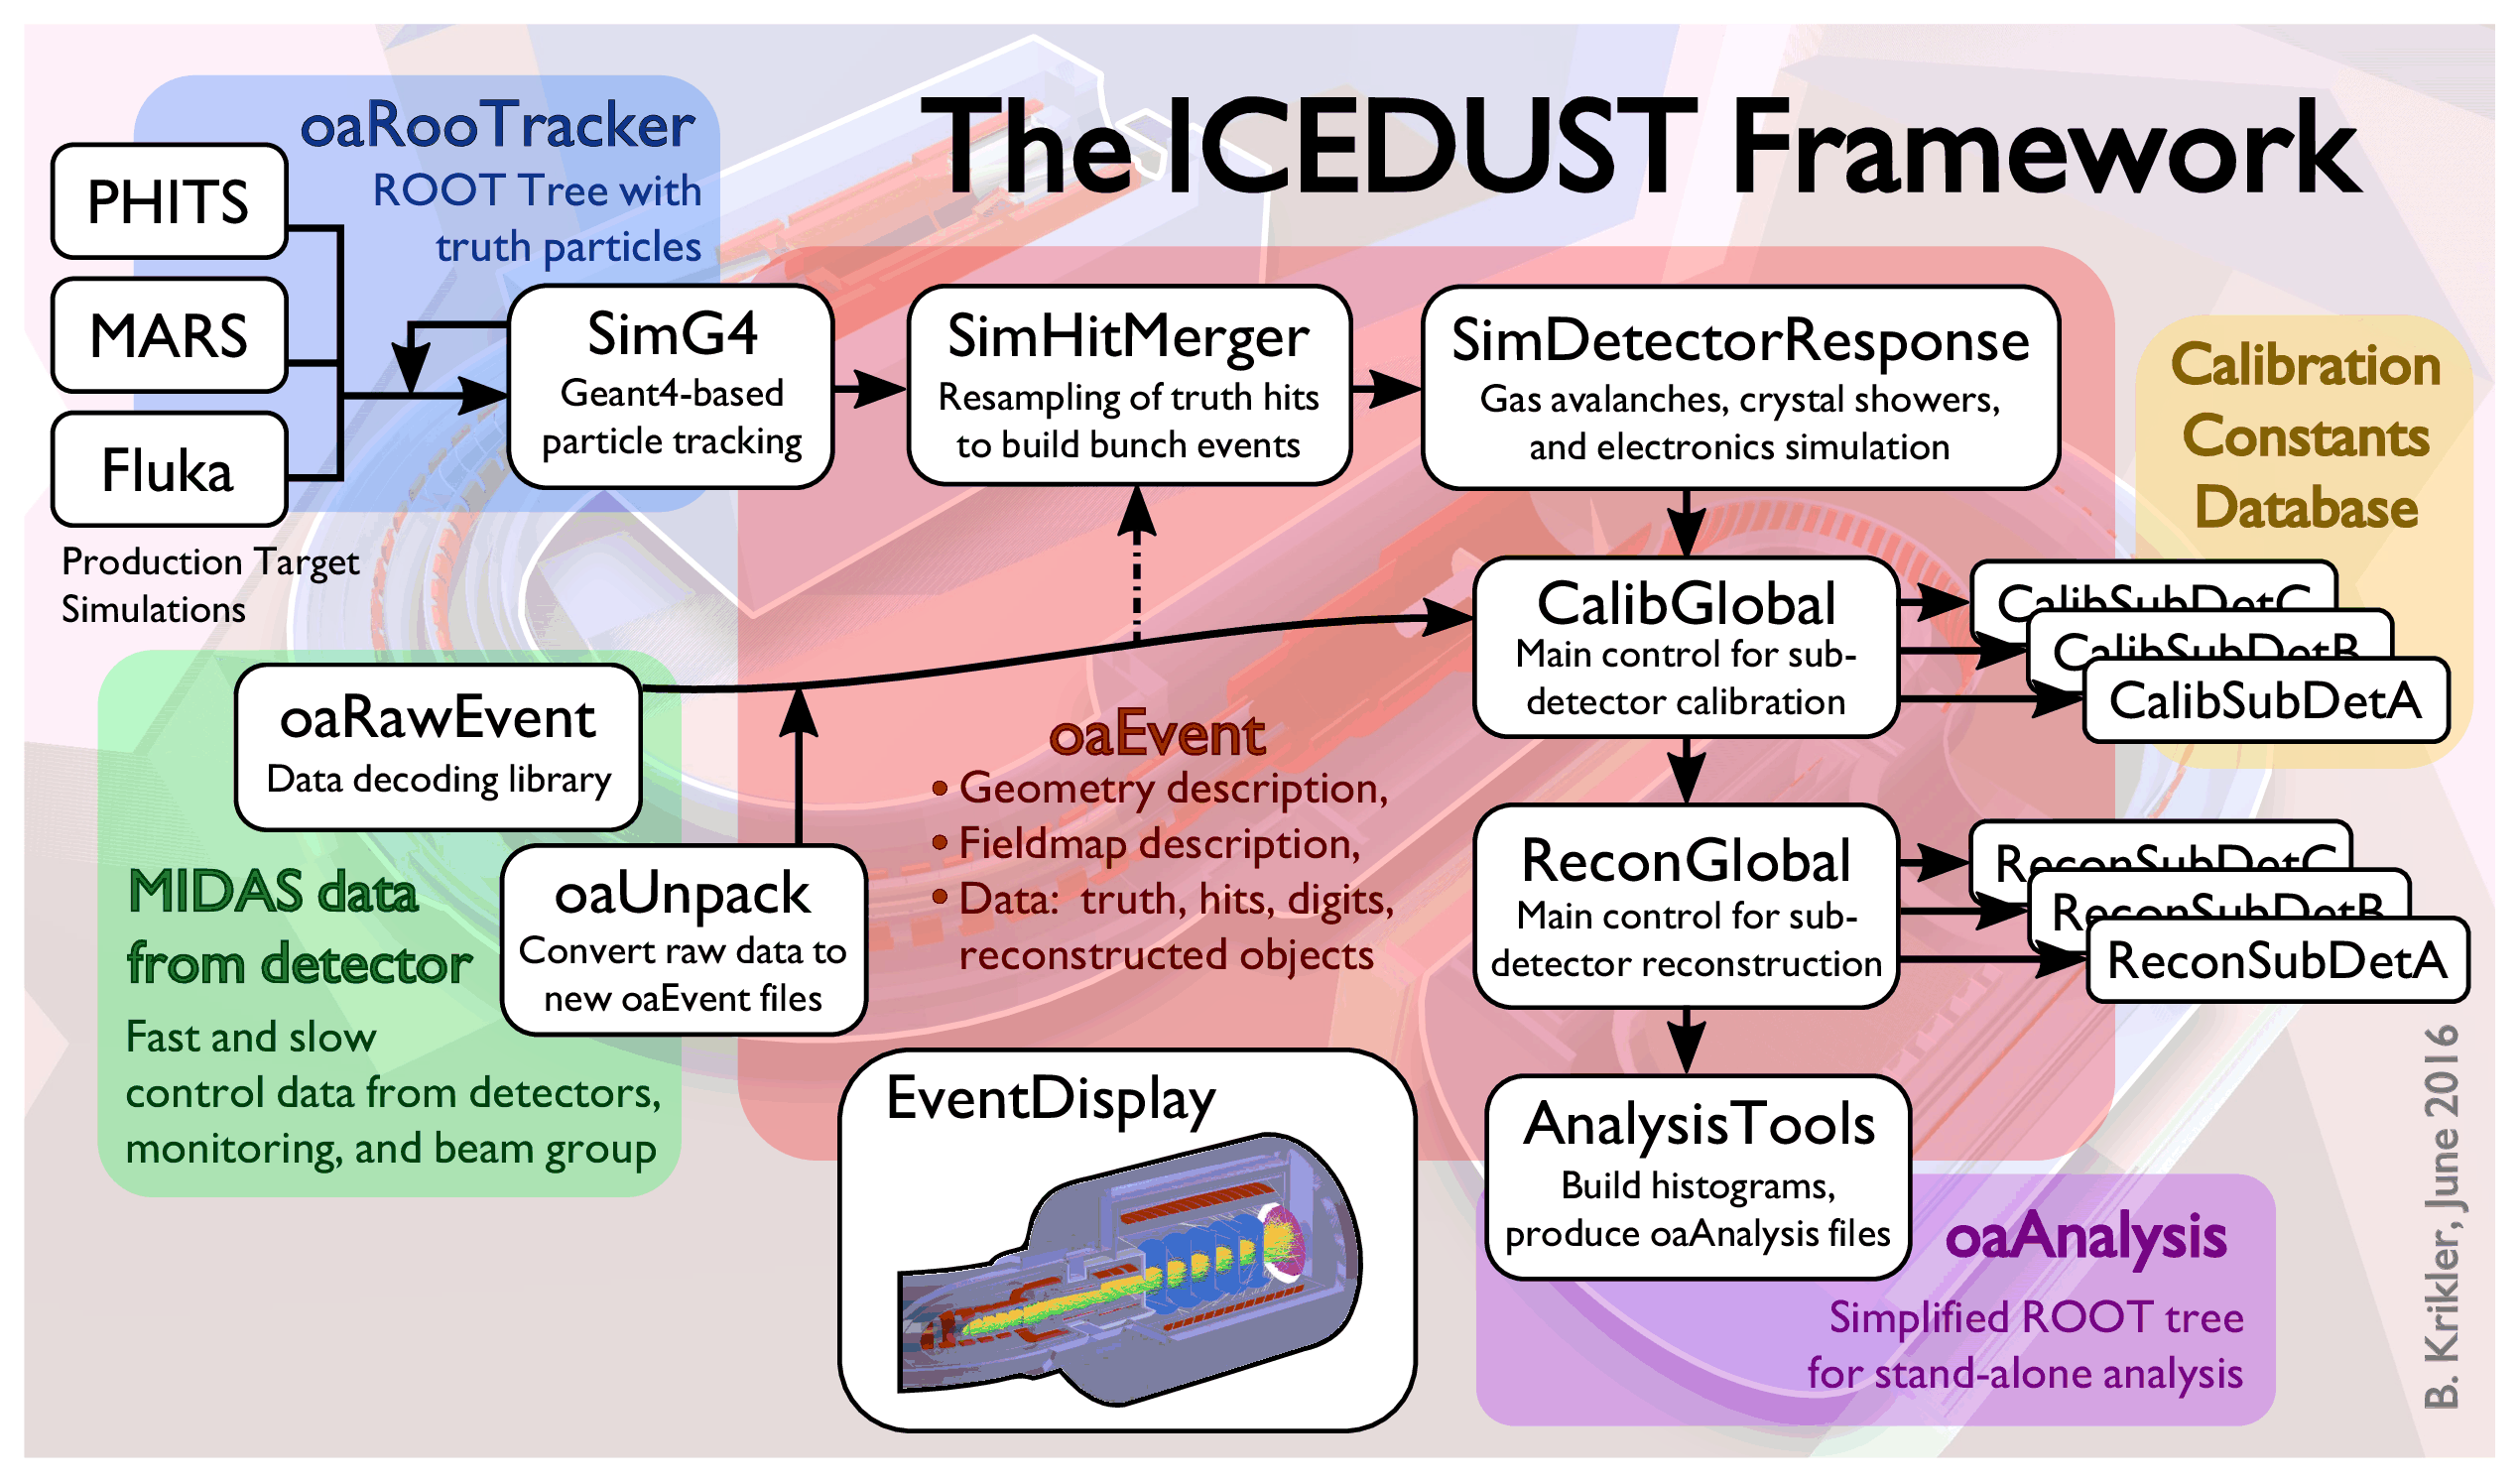
\includegraphics[width=1.00\textwidth,trim=0.85cm 0.5cm 0.5cm 0.5cm,clip=true]{figs/software/ICEDUST_structure}
%}
\caption{
Overview diagram for the ICEDUST framework.
Data produced from simulation or taken in the real experiment are treated identically through the calibration and onwards up to analysis.
}
\figlabel{software:ICEDUSTOverview}
\end{figure}
}

\newcommand{\FigNDTwoEighty}{
\begin{figure}[t]
\centering
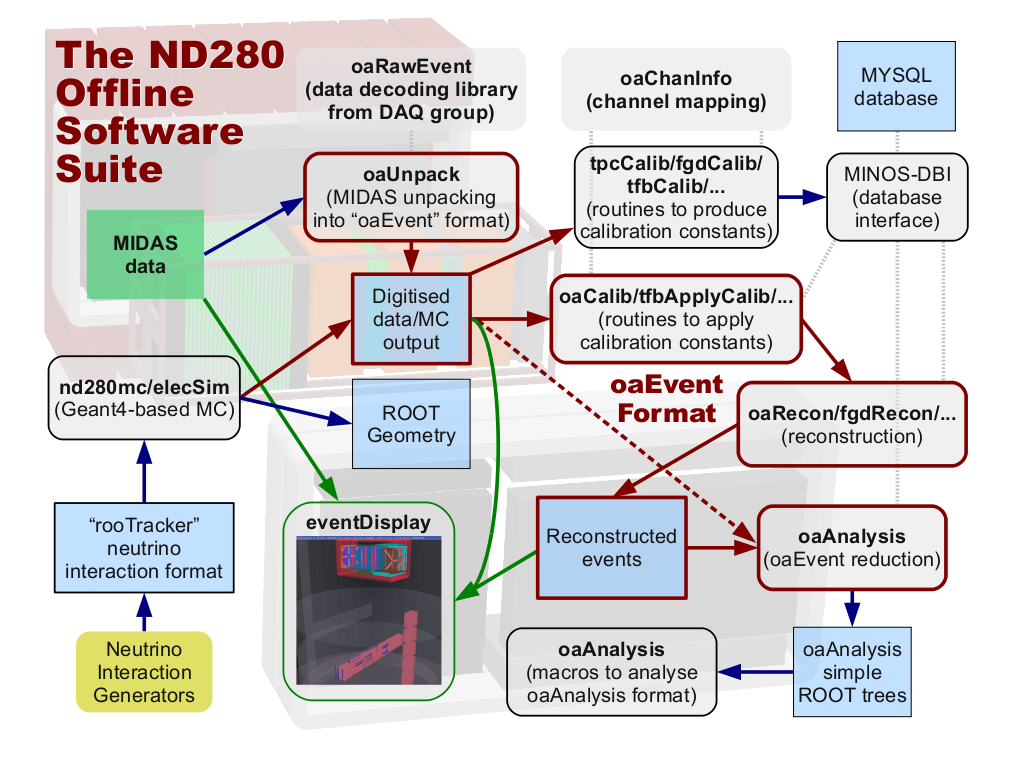
\includegraphics[width=0.95\textwidth]{figs/software/ND280SoftwareDiagram}
\caption{
Overview diagram for the ND280 framework.
}
\figlabel{software:ND280}
\end{figure}
}

\newcommand{\FigSimulationOverview}{
\begin{figure}[t]
\centering
%\fbox{
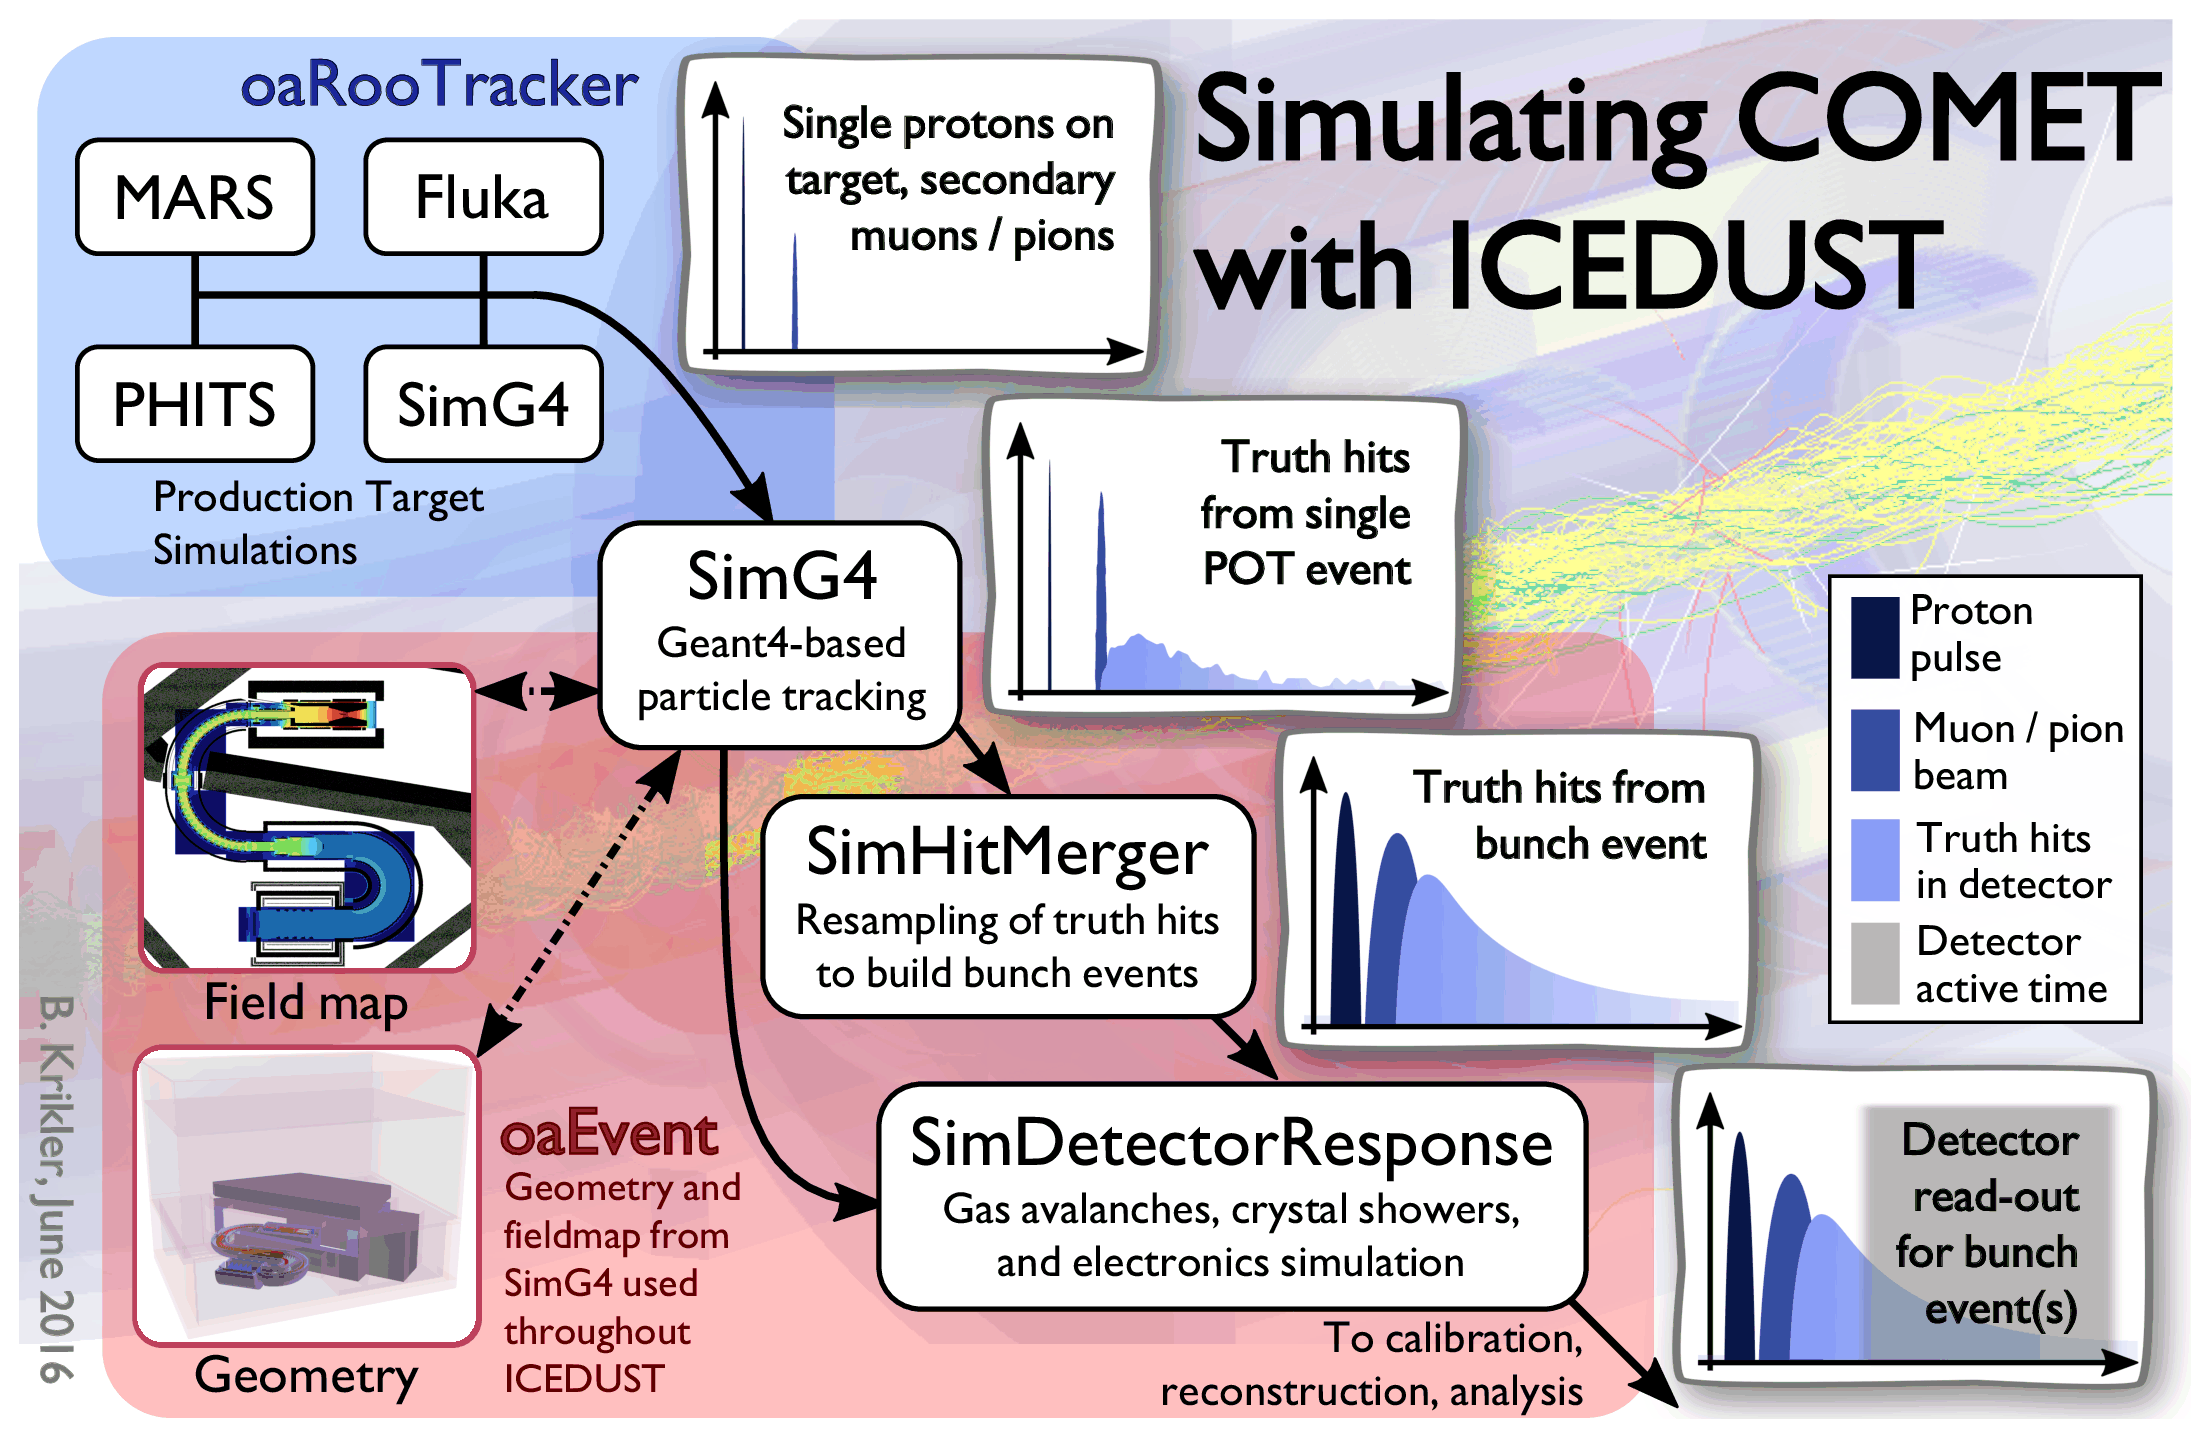
\includegraphics[width=1.00\textwidth]{figs/software/Simulation_structure}
%}
\caption{
Diagram showing the stages used to simulate COMET.
The timing schematics on the right show how a simulated event is built up, firstly by producing many individual proton interactions with the production target,
then by transporting the secondary particles to produce energy deposits in the detector, which are then combined with the truth hits from other proton events to produce a realistic bunch structure.
Finally, these bunch events are processed through the detector response simulation to produce fake waveforms and other detector read-outs.
}
\figlabel{software:SimulationOverview}
\end{figure}
}

\newcommand{\FigGeometryHeirarchy}{
\begin{figure}[t]
\centering
%\fbox{
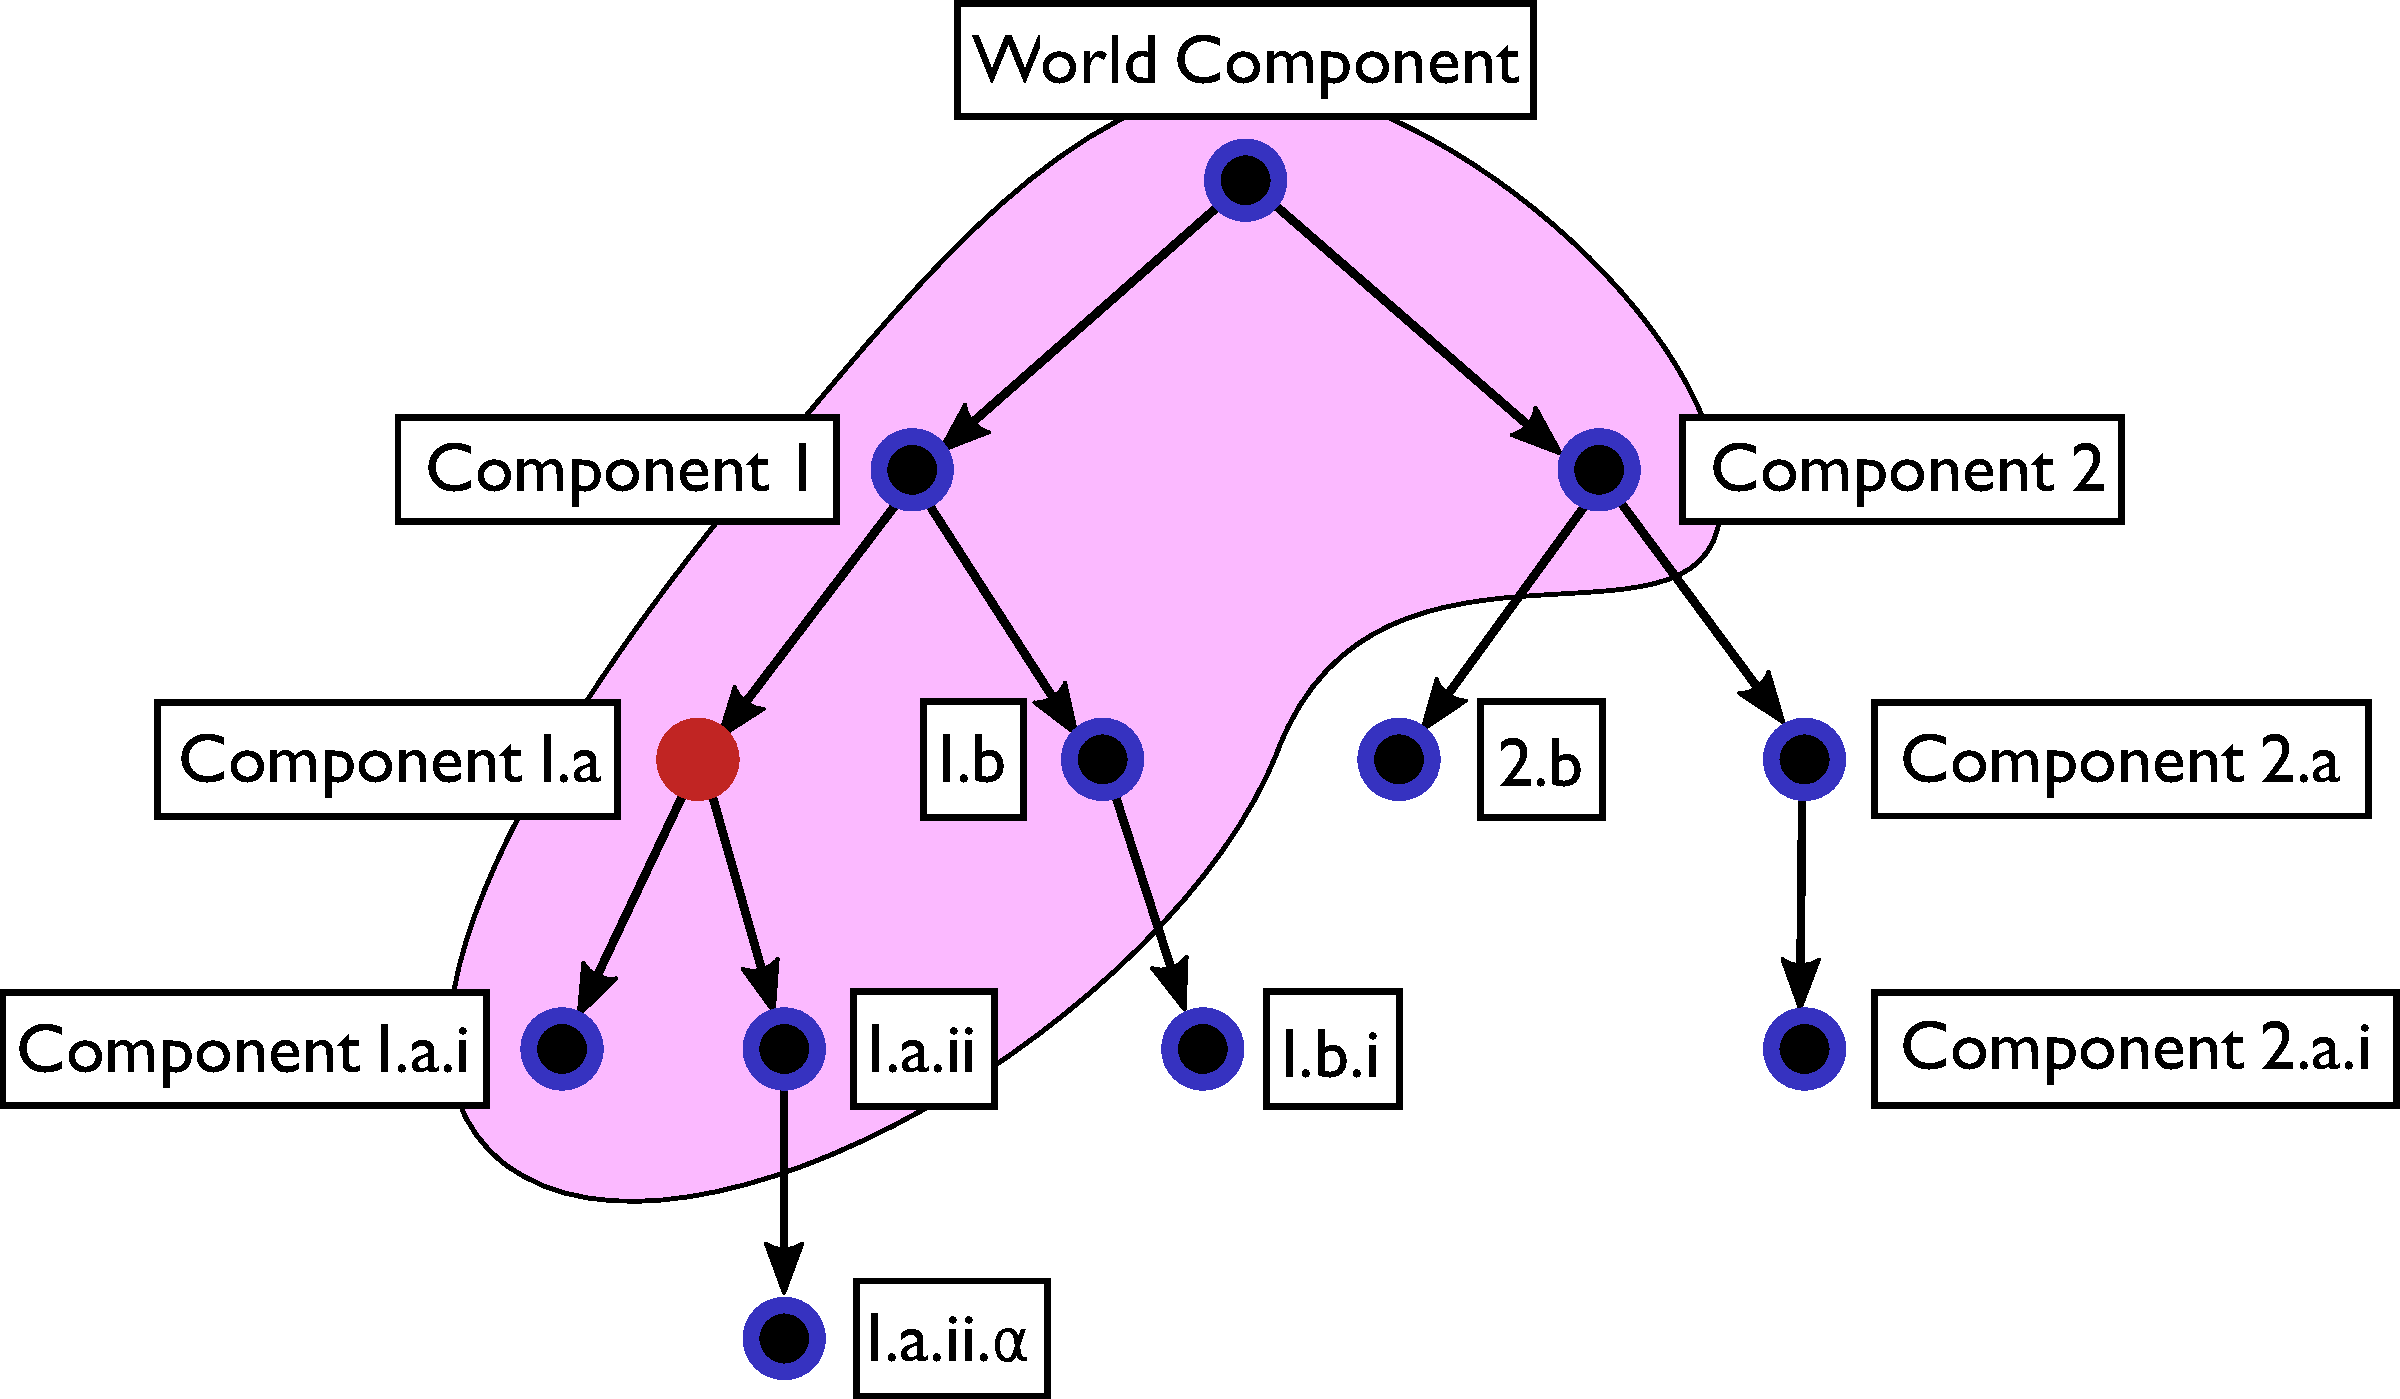
\includegraphics[width=0.70\textwidth]{figs/software/ComponentHeirarchy}
%}
\caption{
How parameters are shared amongst different components.
Parameters of component 1.a (in red) can access the value of parameters owned by components contained in the larger violet region.
}
\figlabel{software:componentHeirarchy}
\end{figure}
}

\newcommand{\FigGeometryParameters}{
\begin{figure}[t]
\lstinputlisting[style=customc]{figs/software/demo-parameters.mac}
\caption{
An example set of parameter definitions which control the geometry for the Torus2.
Parameter specifications use natural arithmetic notation and can reference other parameters and use standard units.
They can also be formed as sets where each element has a different value, such as the \texttt{Coils:Position} parameter.
}
\figlabel{software:geom:paramAssignments}
\end{figure}
}

\newcommand{\FigGeometryScreenshots}{
\begin{figure}[tb]
        \subfloat[][\figlabel{software:geom:screenshots:phaseI}\phaseI]  {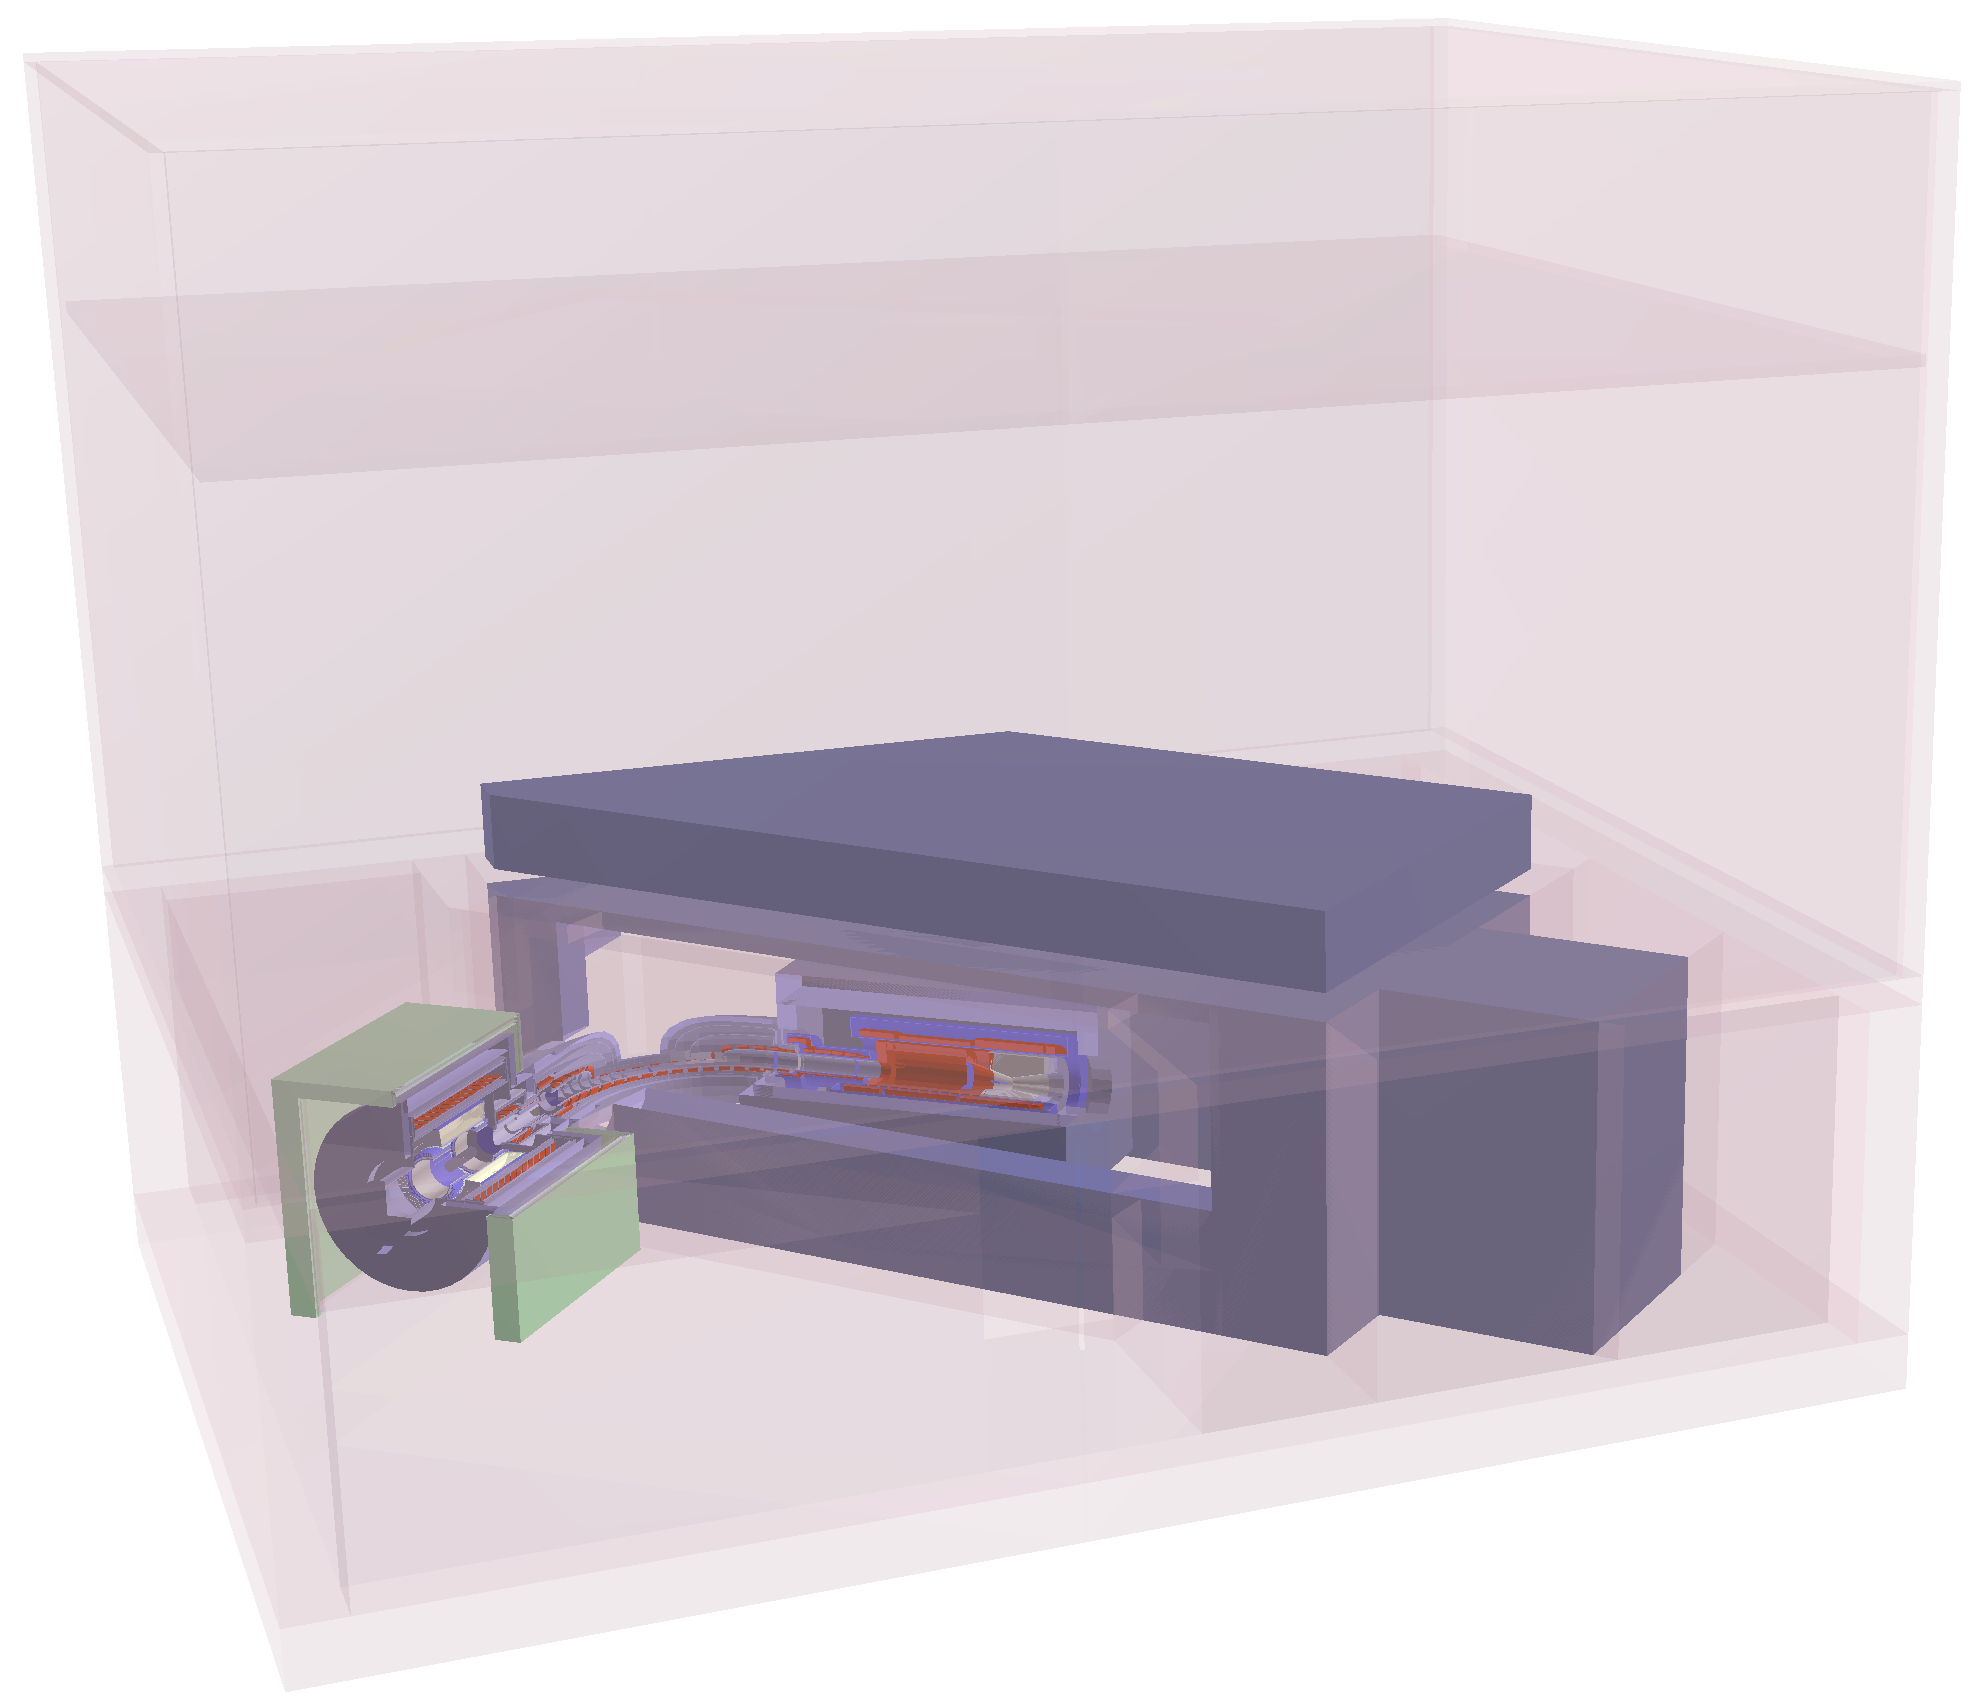
\includegraphics[height=0.25\textheight]{figs/software/Phase-I-UpdateGeom}}\hspace{2ex}%
        \subfloat[][\figlabel{software:geom:screenshots:phaseII}\phaseII]{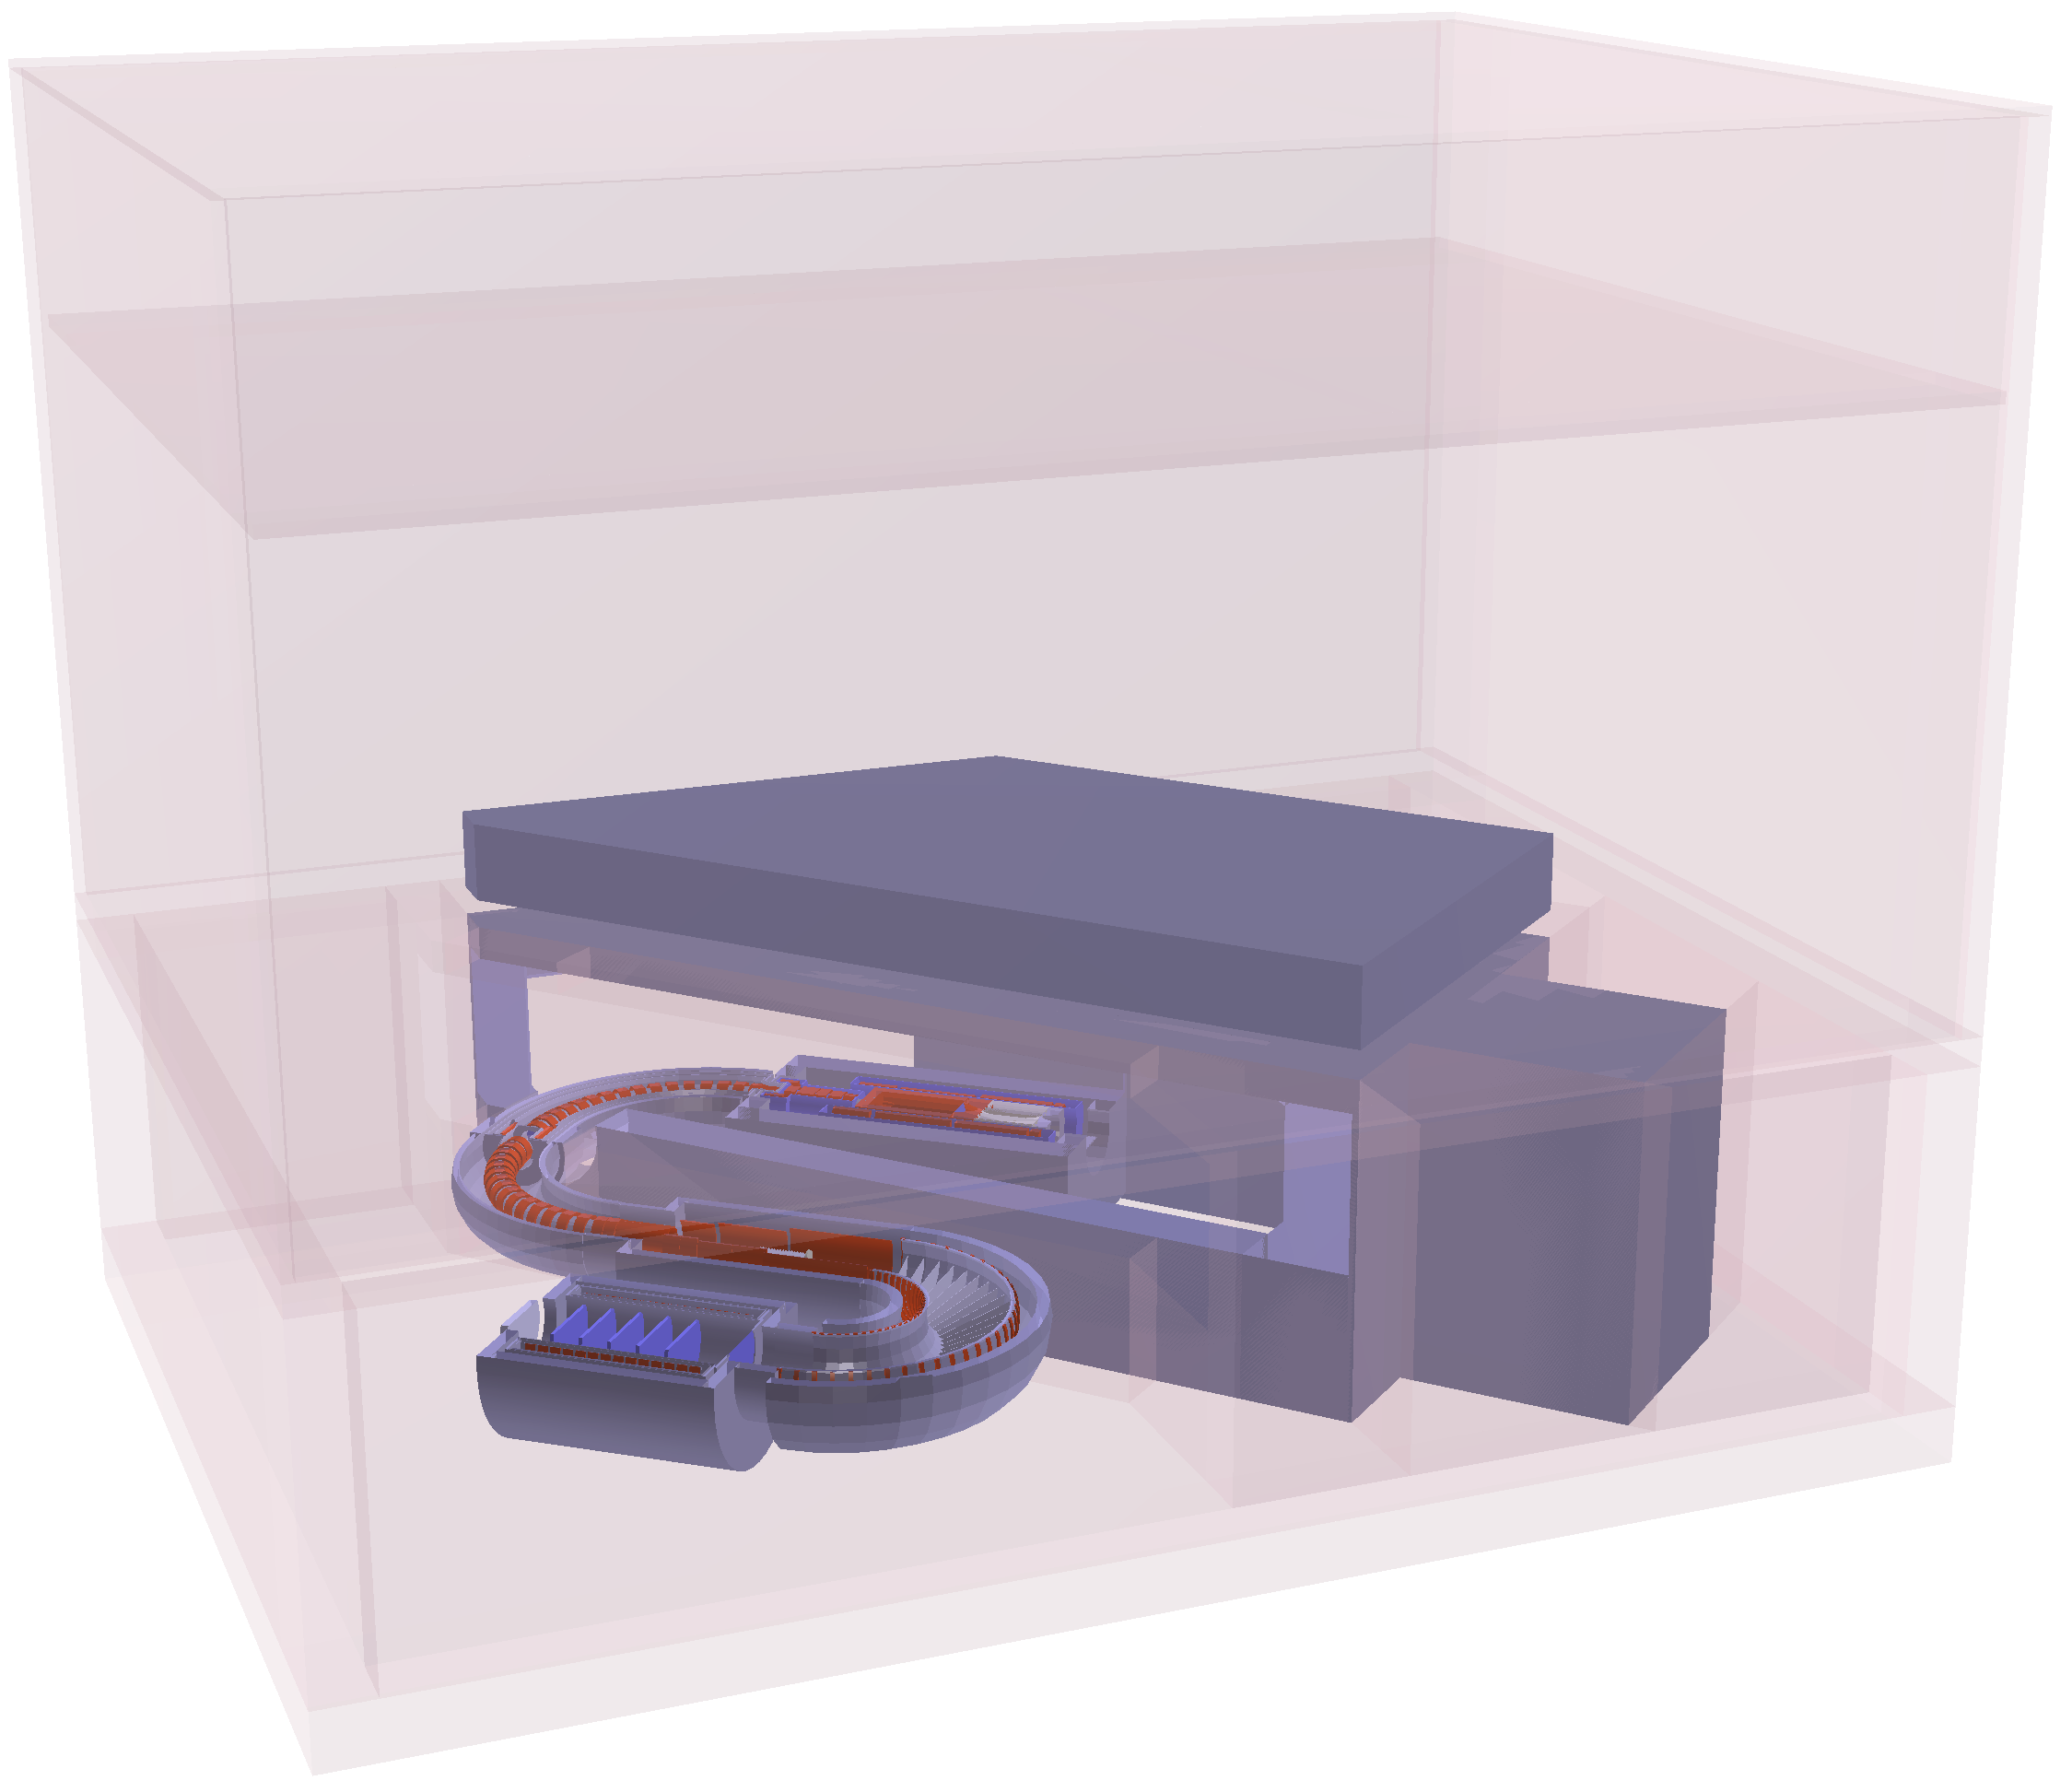
\includegraphics[height=0.25\textheight,trim=0 0.3cm 0 2.6cm,clip=true]{figs/software/Phase-II-UpdateGeom.png}}
\caption{\figlabel{software:geom:screenshots} %
Two of the possible simulation `worlds' that can be selected at run-time:
        \protect\subref{fig:software:geom:screenshots:phaseI} \phaseI with the CyDet detector installed, and
        \protect\subref{fig:software:geom:screenshots:phaseII} \phaseII.  
	Mutiple \phaseI worlds exist, one for each potential running configuration.
}
\end{figure}
}

\newcommand{\FigPiYieldHadronCodes}{
\begin{figure}[b]
\centering
%\fbox{
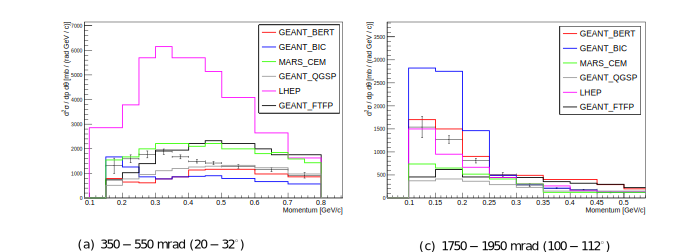
\includegraphics[width=0.95\textwidth,trim=2cm 1cm 0.8cm 0.5cm,clip=true]{figs/software/PionYield_AEdmondsThesis}
%}
\caption{
Comparison of various hadron production codes with experimental data from the HARP experiment, taken from the thesis of A. Edmonds~\cite{AEdmondsThesis}.
Points with error bars are the experimental data.  Left: double differential-production cross-section for pion production from 20 to 32\degree with respect to the incoming proton direction; right: from 100 to 112\degree.
The hadron production code that best reproduces the data depends strongly on the angular region under consideration.
}
\figlabel{software:piYield}
\end{figure}
}

\newcommand{\FigSoftwarePhysicsSpectra}{
\begin{figure}[p]
\centering
%\fbox{
\subfloat[][\figlabel{software:customPhysic:DIO}Electrons from $\mu$ Decay-in-Orbit]{
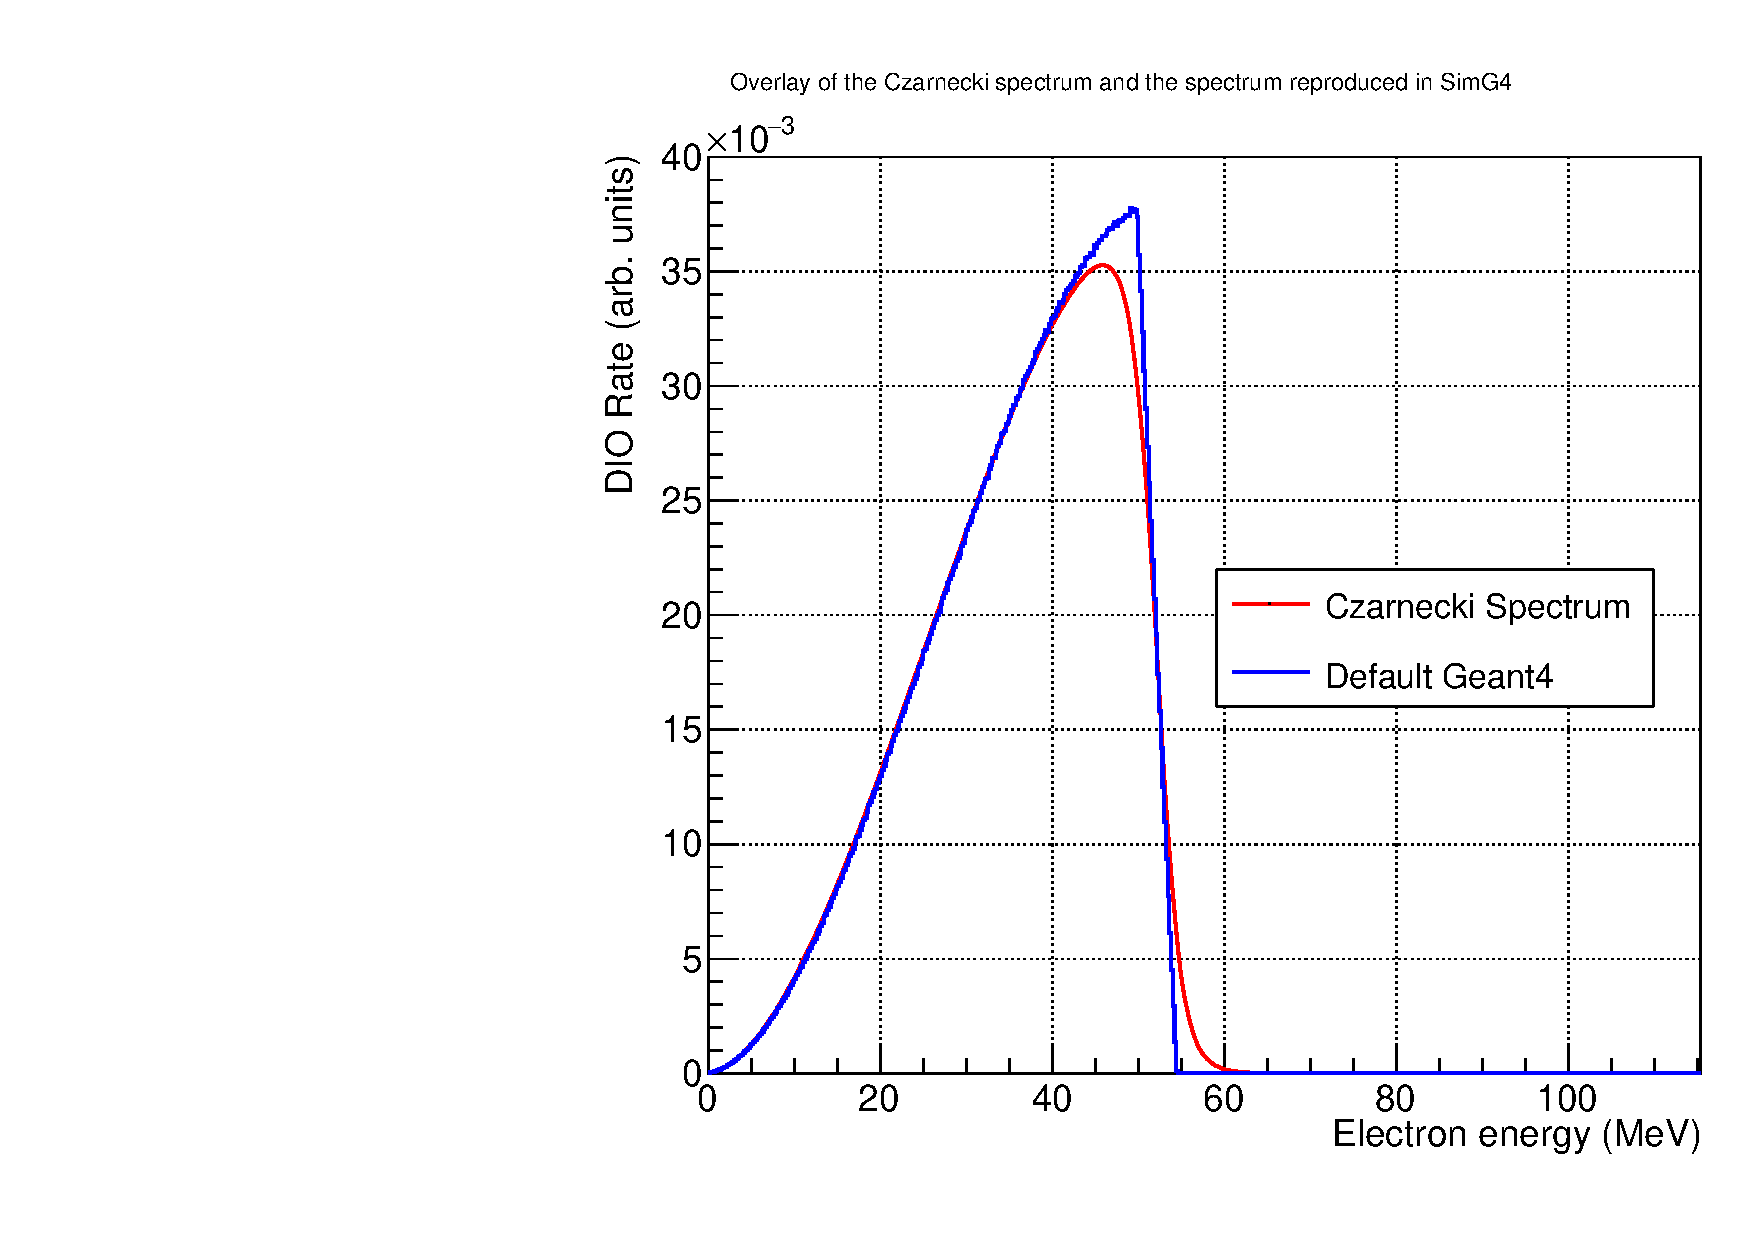
\includegraphics[width=0.45\textwidth,trim=0cm 0cm 0.0cm 1.3cm,clip=true]{figs/software/160822_BoundDecay_Geant4_vs_Czarnecki-lin.pdf}
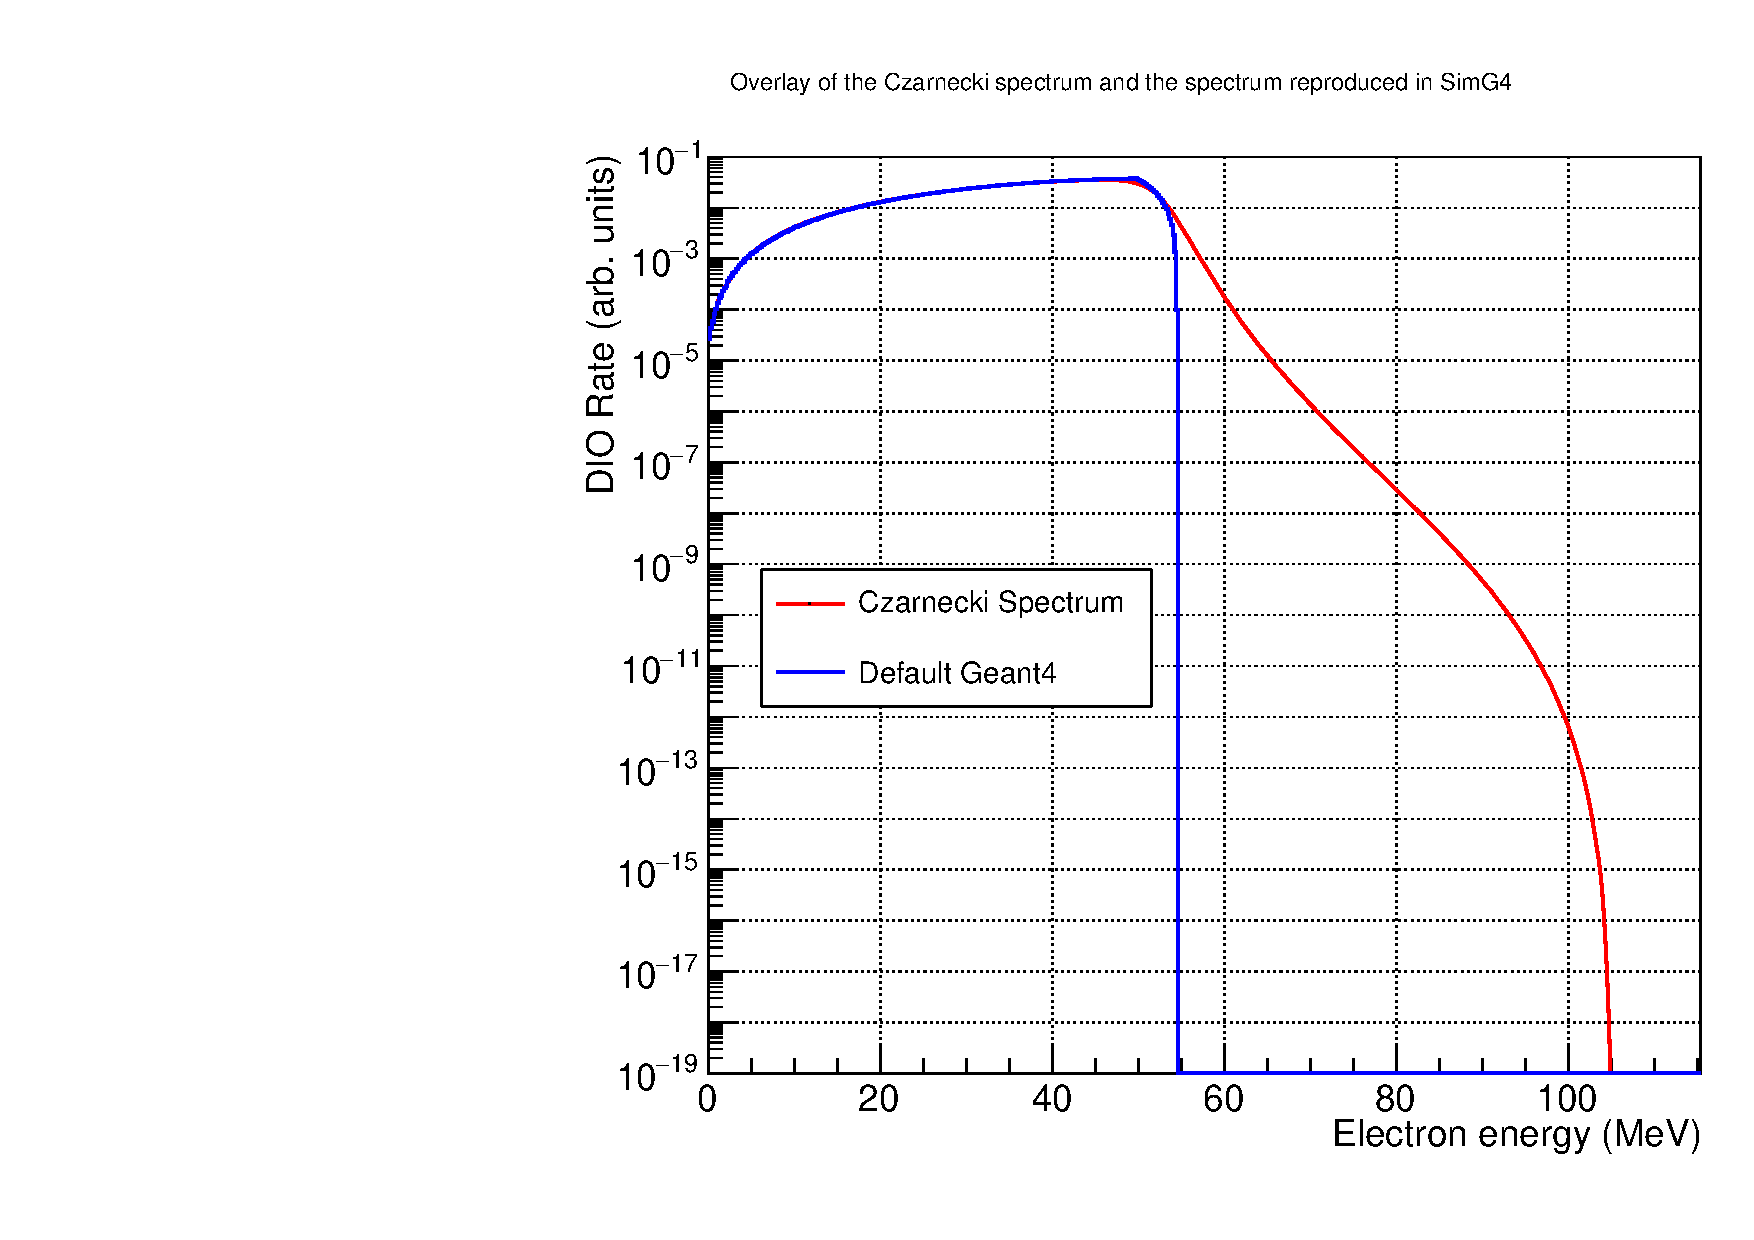
\includegraphics[width=0.45\textwidth,trim=0cm 0cm 0.0cm 1.3cm,clip=true]{figs/software/160822_BoundDecay_Geant4_vs_Czarnecki-log.pdf}
}\\
\subfloat[][\figlabel{software:customPhysic:ProtMuCap}Protons Emitted Following $\mu$ Nuclear Capture]{
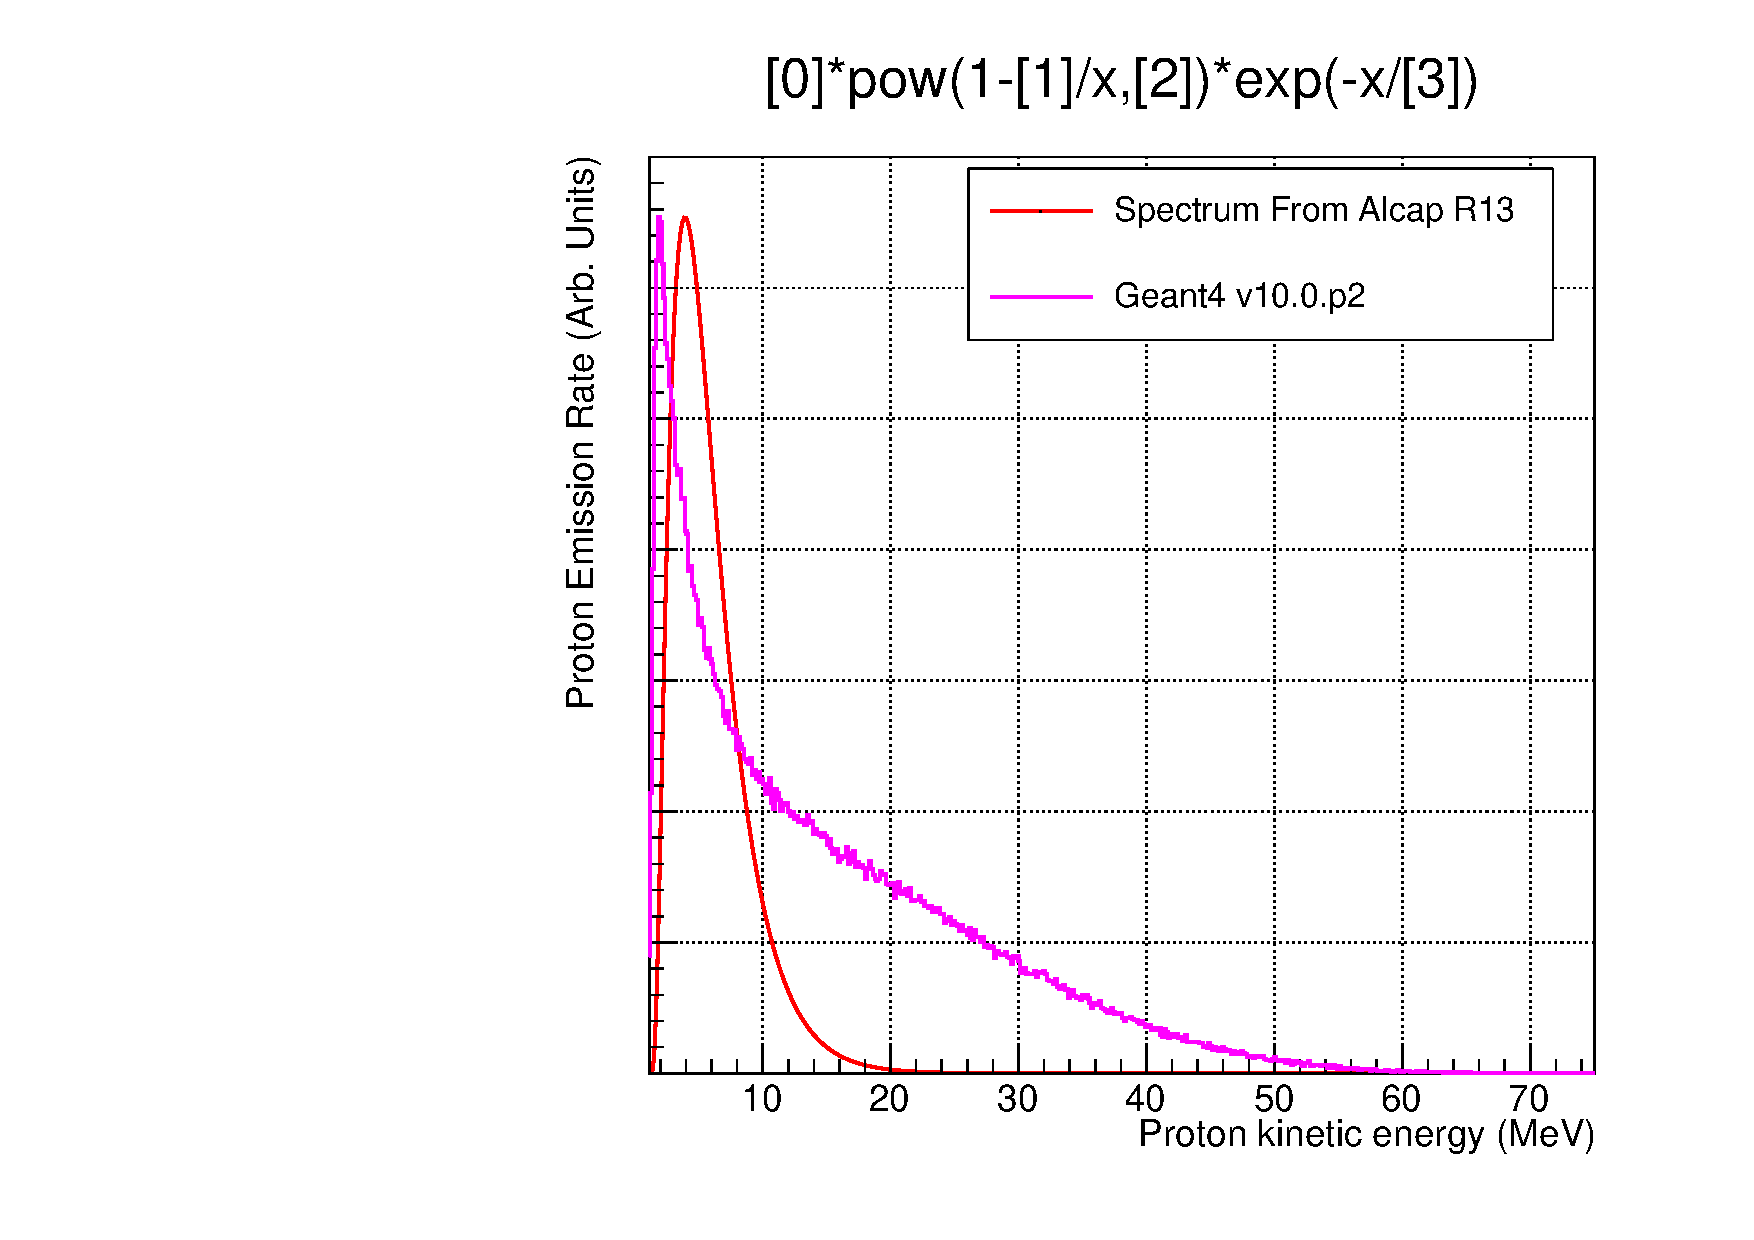
\includegraphics[width=0.45\textwidth,trim=0cm 0cm 1.8cm 1.9cm,clip=true]{figs/software/160822_Geant4VsAlcap-lin.pdf}
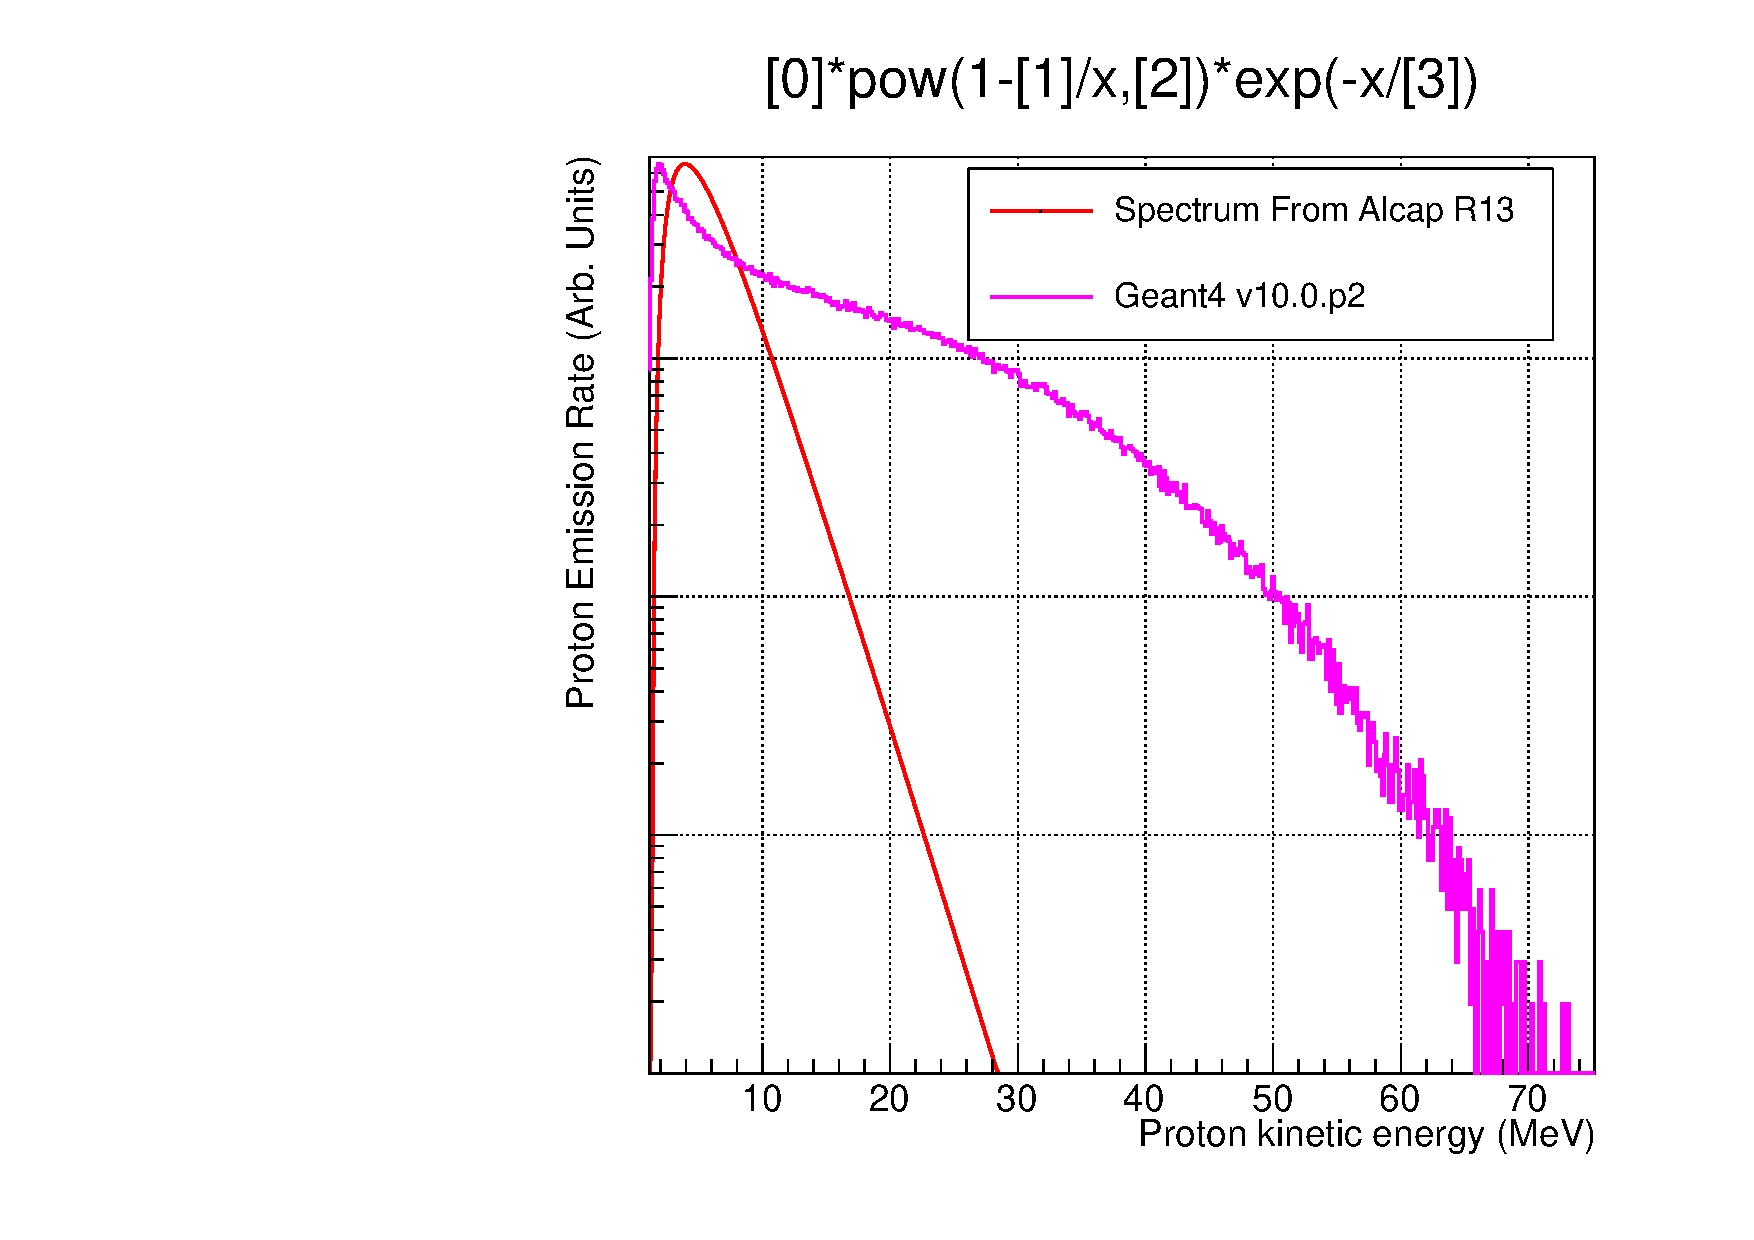
\includegraphics[width=0.45\textwidth,trim=0cm 0cm 1.8cm 1.9cm,clip=true]{figs/software/160822_Geant4VsAlcap-log.pdf}
}
%}
\caption{
\figlabel{software:customPhysic}
Comparison of the realistic spectra for \ac{DIO} electrons, \protect\subref{fig:software:customPhysic:DIO} (normalised to agree at 35~MeV), and protons coming from muon nuclear capture, \protect\subref{fig:software:customPhysic:ProtMuCap} (normalised to have the same maximum value), each on a linear scale (left) and a logarithmic scale (right).
The \ac{DIO} spectrum used in default Geant4 has a sharp cut-off slightly above the free muon decay end-point, to be compared with the long but steeply falling tail of the Czarnecki \etal theoretical calculation~\cite{Czarnecki2011}.
The comparison of protons coming from muon capture between the preliminary result from AlCap and default Geant4 shows that the true proton spectrum is much softer than the Geant4 model.
}
\end{figure}
}

\newcommand{\FigSimulationPhysicsClasses}{
\begin{figure}[tb]
\centering
%\fbox{
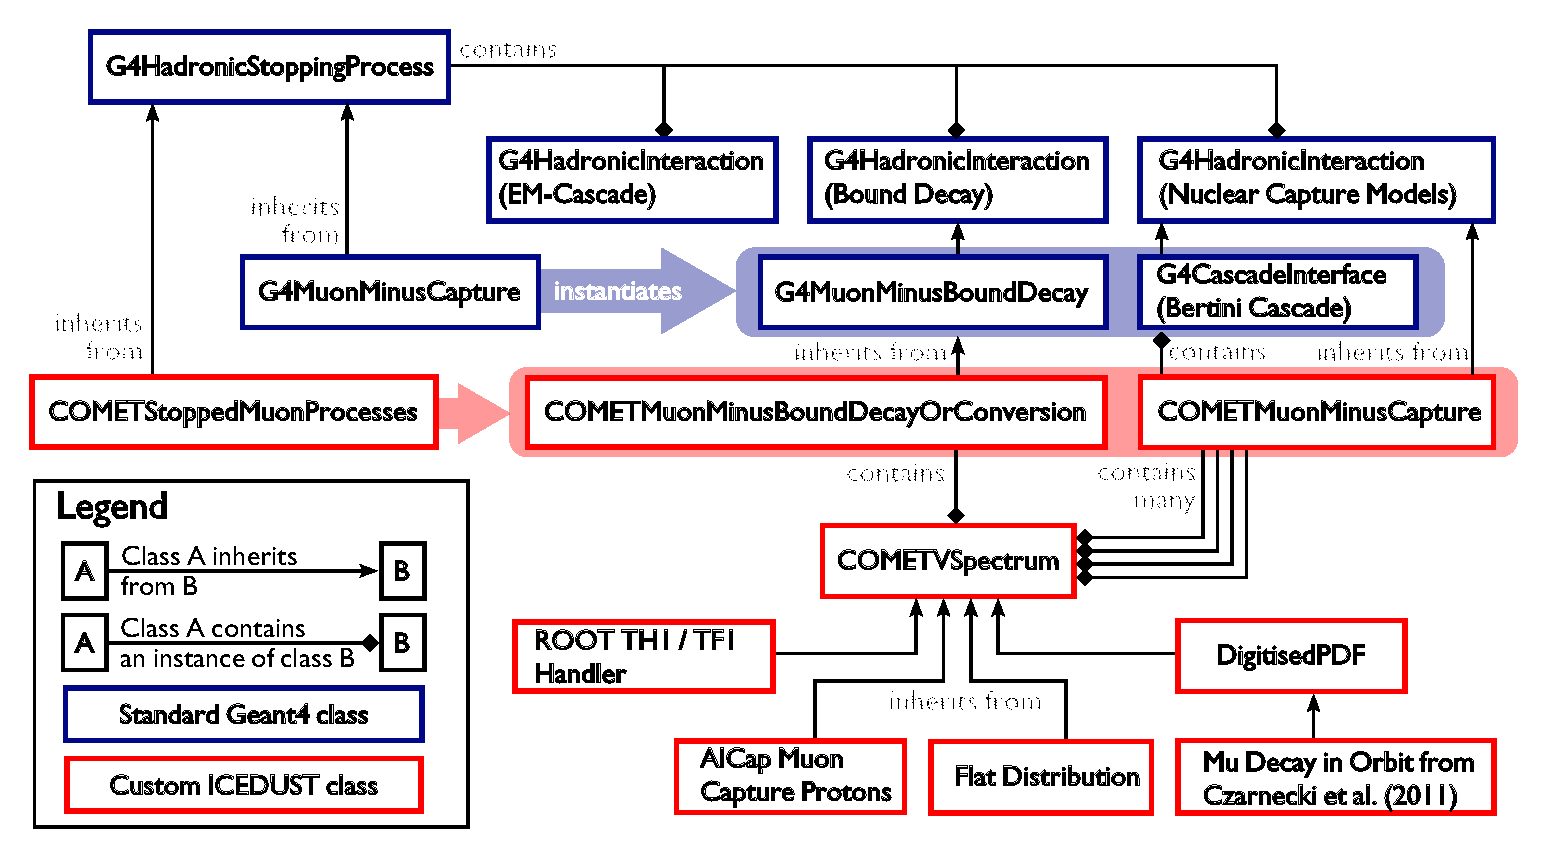
\includegraphics[width=1.00\textwidth]{figs/software/SimulationMuonPhysicsClasses}
%}
\caption{
The various classes involved in simulating the various processes of stopped negative muons.
%Classes in red have been implemented for COMET and augment the existing Geant4 classes which are shown in blue.
The standard Geant4 model is activated by registering `G4MuonMinusCapture', which instantiates `G4MuonMinusBoundDecay' and `G4CascadeInterface' to run the \ac{DIO} and nuclear capture respectively.
To use the custom COMET muon physics, an instance of `COMETStoppedMuonProcess' should be registered, which sets up `COMETMuonMinusBoundDecayOrConversion' to produce the electron (and possibly neutrinos) from \ac{DIO} or conversion, and `COMETMuonMinusCapture' to do the nuclear capture.
}
\figlabel{software:ExtendedMuonClasses}
\end{figure}
}

\newcommand{\FigSoftwareFieldMap}{
\begin{figure}[b]
\centering
%\fbox{
\subfloat[][\figlabel{software:field:Opera}Opera calculation]{
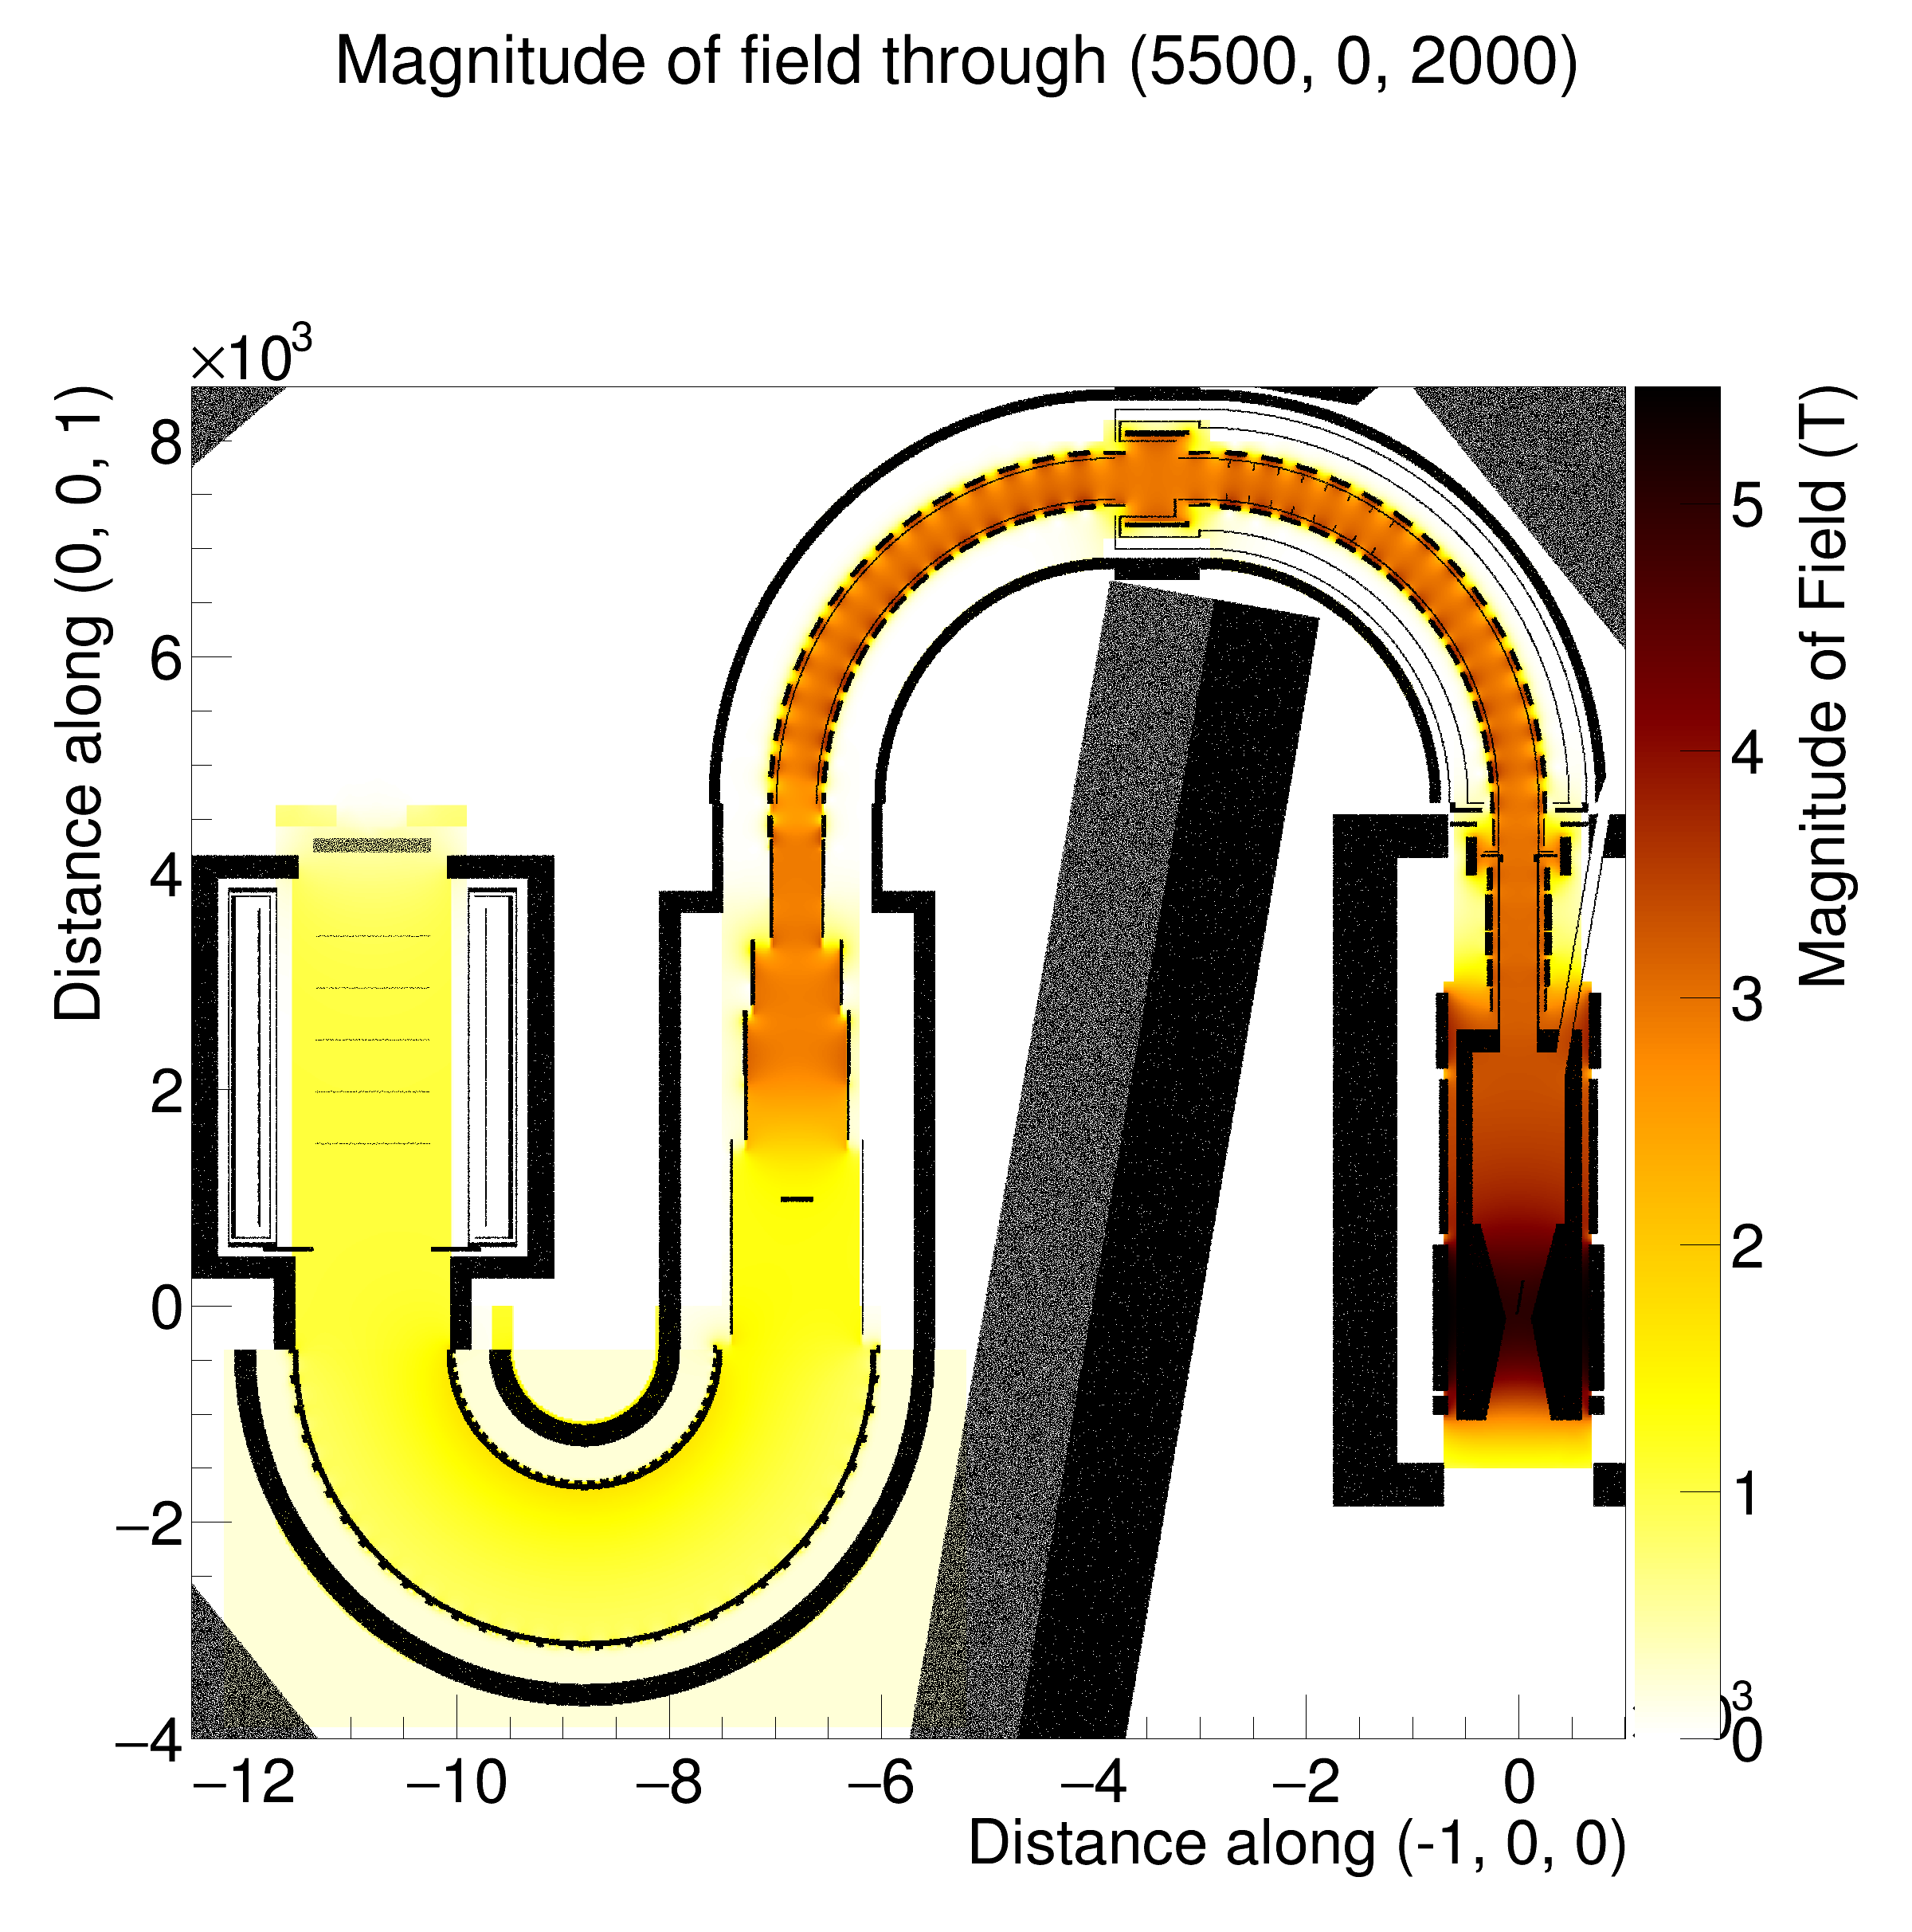
\includegraphics[width=0.45\textwidth,trim=0cm 0cm 0.0cm 13cm,clip=true]{figs/software/Plot_Opera.png}
}
\subfloat[][\figlabel{software:field:G4Beamline}G4Beamline calculation]{
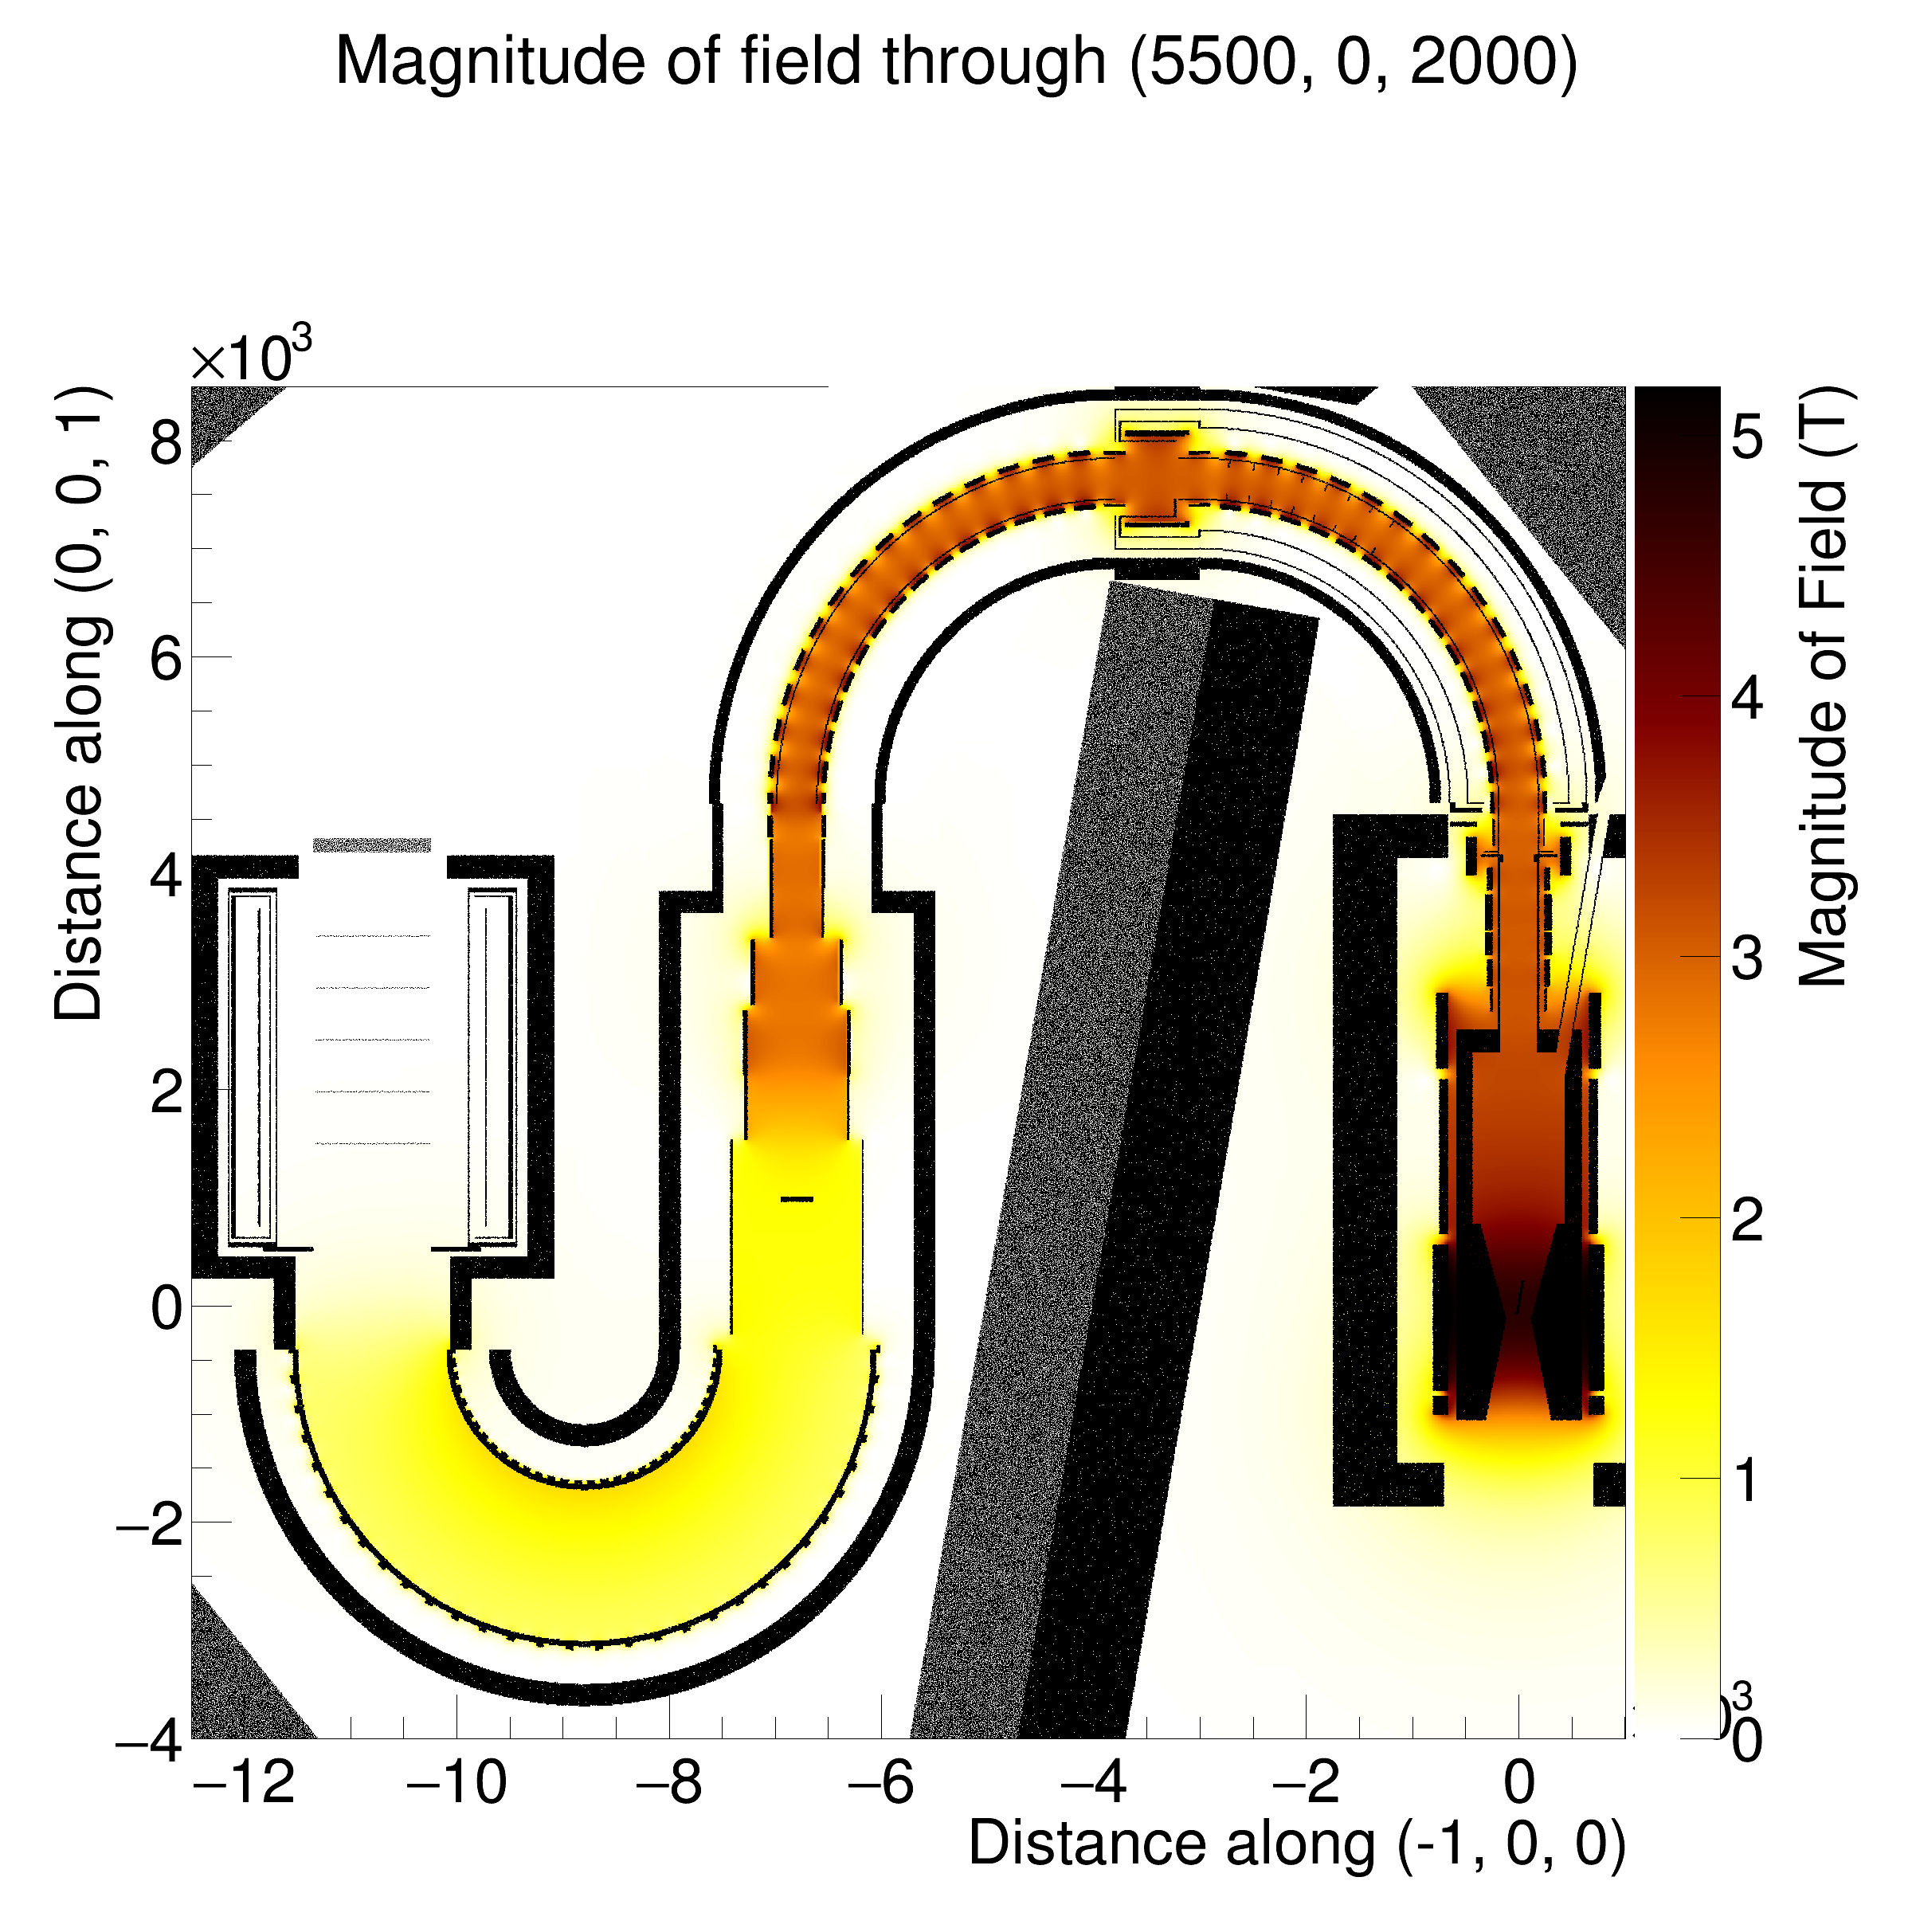
\includegraphics[width=0.45\textwidth,trim=0cm 0cm 0.0cm 13cm,clip=true]{figs/software/Plot_G4Beamline.png}
}
%}
\caption{
\figlabel{software:field}
Fieldmap produced by \protect\subref{fig:software:field:Opera} Opera and \protect\subref{fig:software:field:G4Beamline} G4Beamline.
Although the fringe field is larger with the G4Beamline calculation, the lack of material effects make this calculation less reliable.
Note that the G4Beamline calculation does not include the detector solenoid.
}
\end{figure}
}

\newcommand{\FigSoftwareFieldMapComparison}{
\begin{figure}[t]
\centering
%\fbox{
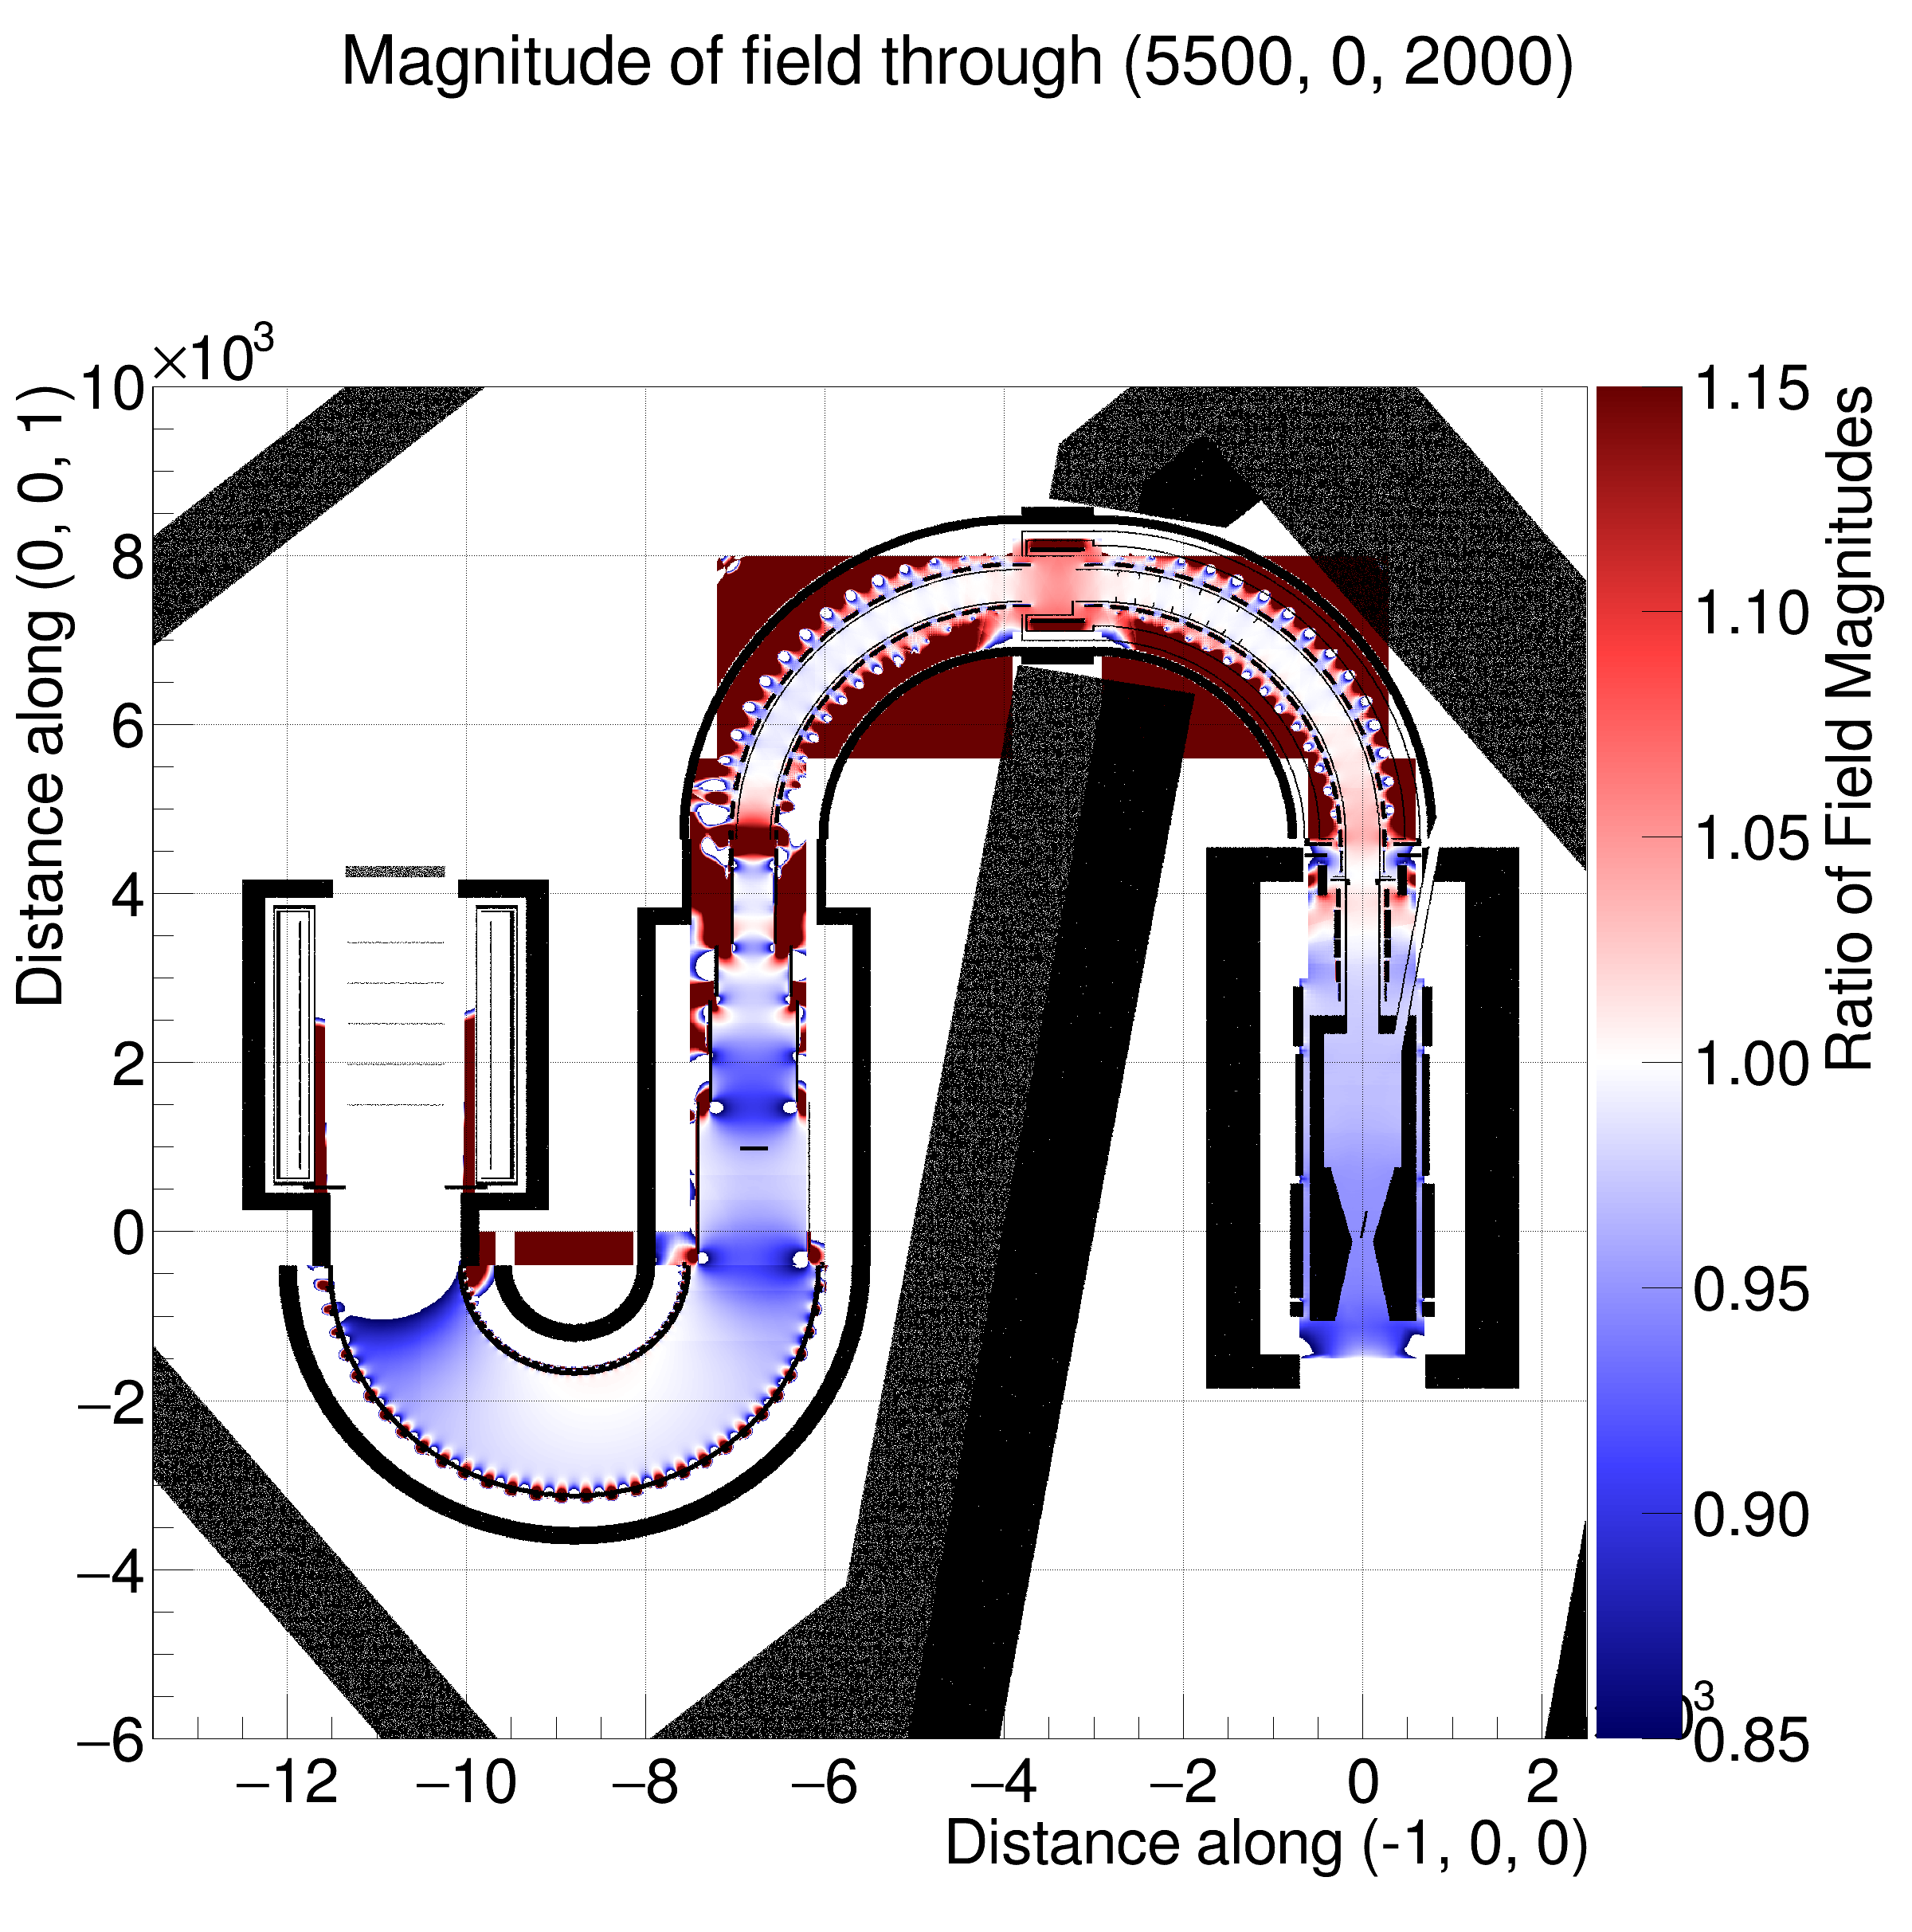
\includegraphics[width=0.9\textwidth,trim=0cm 0cm 0.0cm 13cm,clip=true]{figs/software/Plot_ratio_opera-G4Beamline.png}
%}
\caption{
\figlabel{software:field:comparison}
The ratio of the Opera and G4Beamline calculations shown in \fig{software:field}.
For most of the field within the beamline the calculations agree within 10\%, although around the ends of the solenoids the agreement is poorer.
}
\end{figure}
}

\newcommand{\FigSoftwareDipoleField}{
\begin{figure}[t]
\centering
%\fbox{
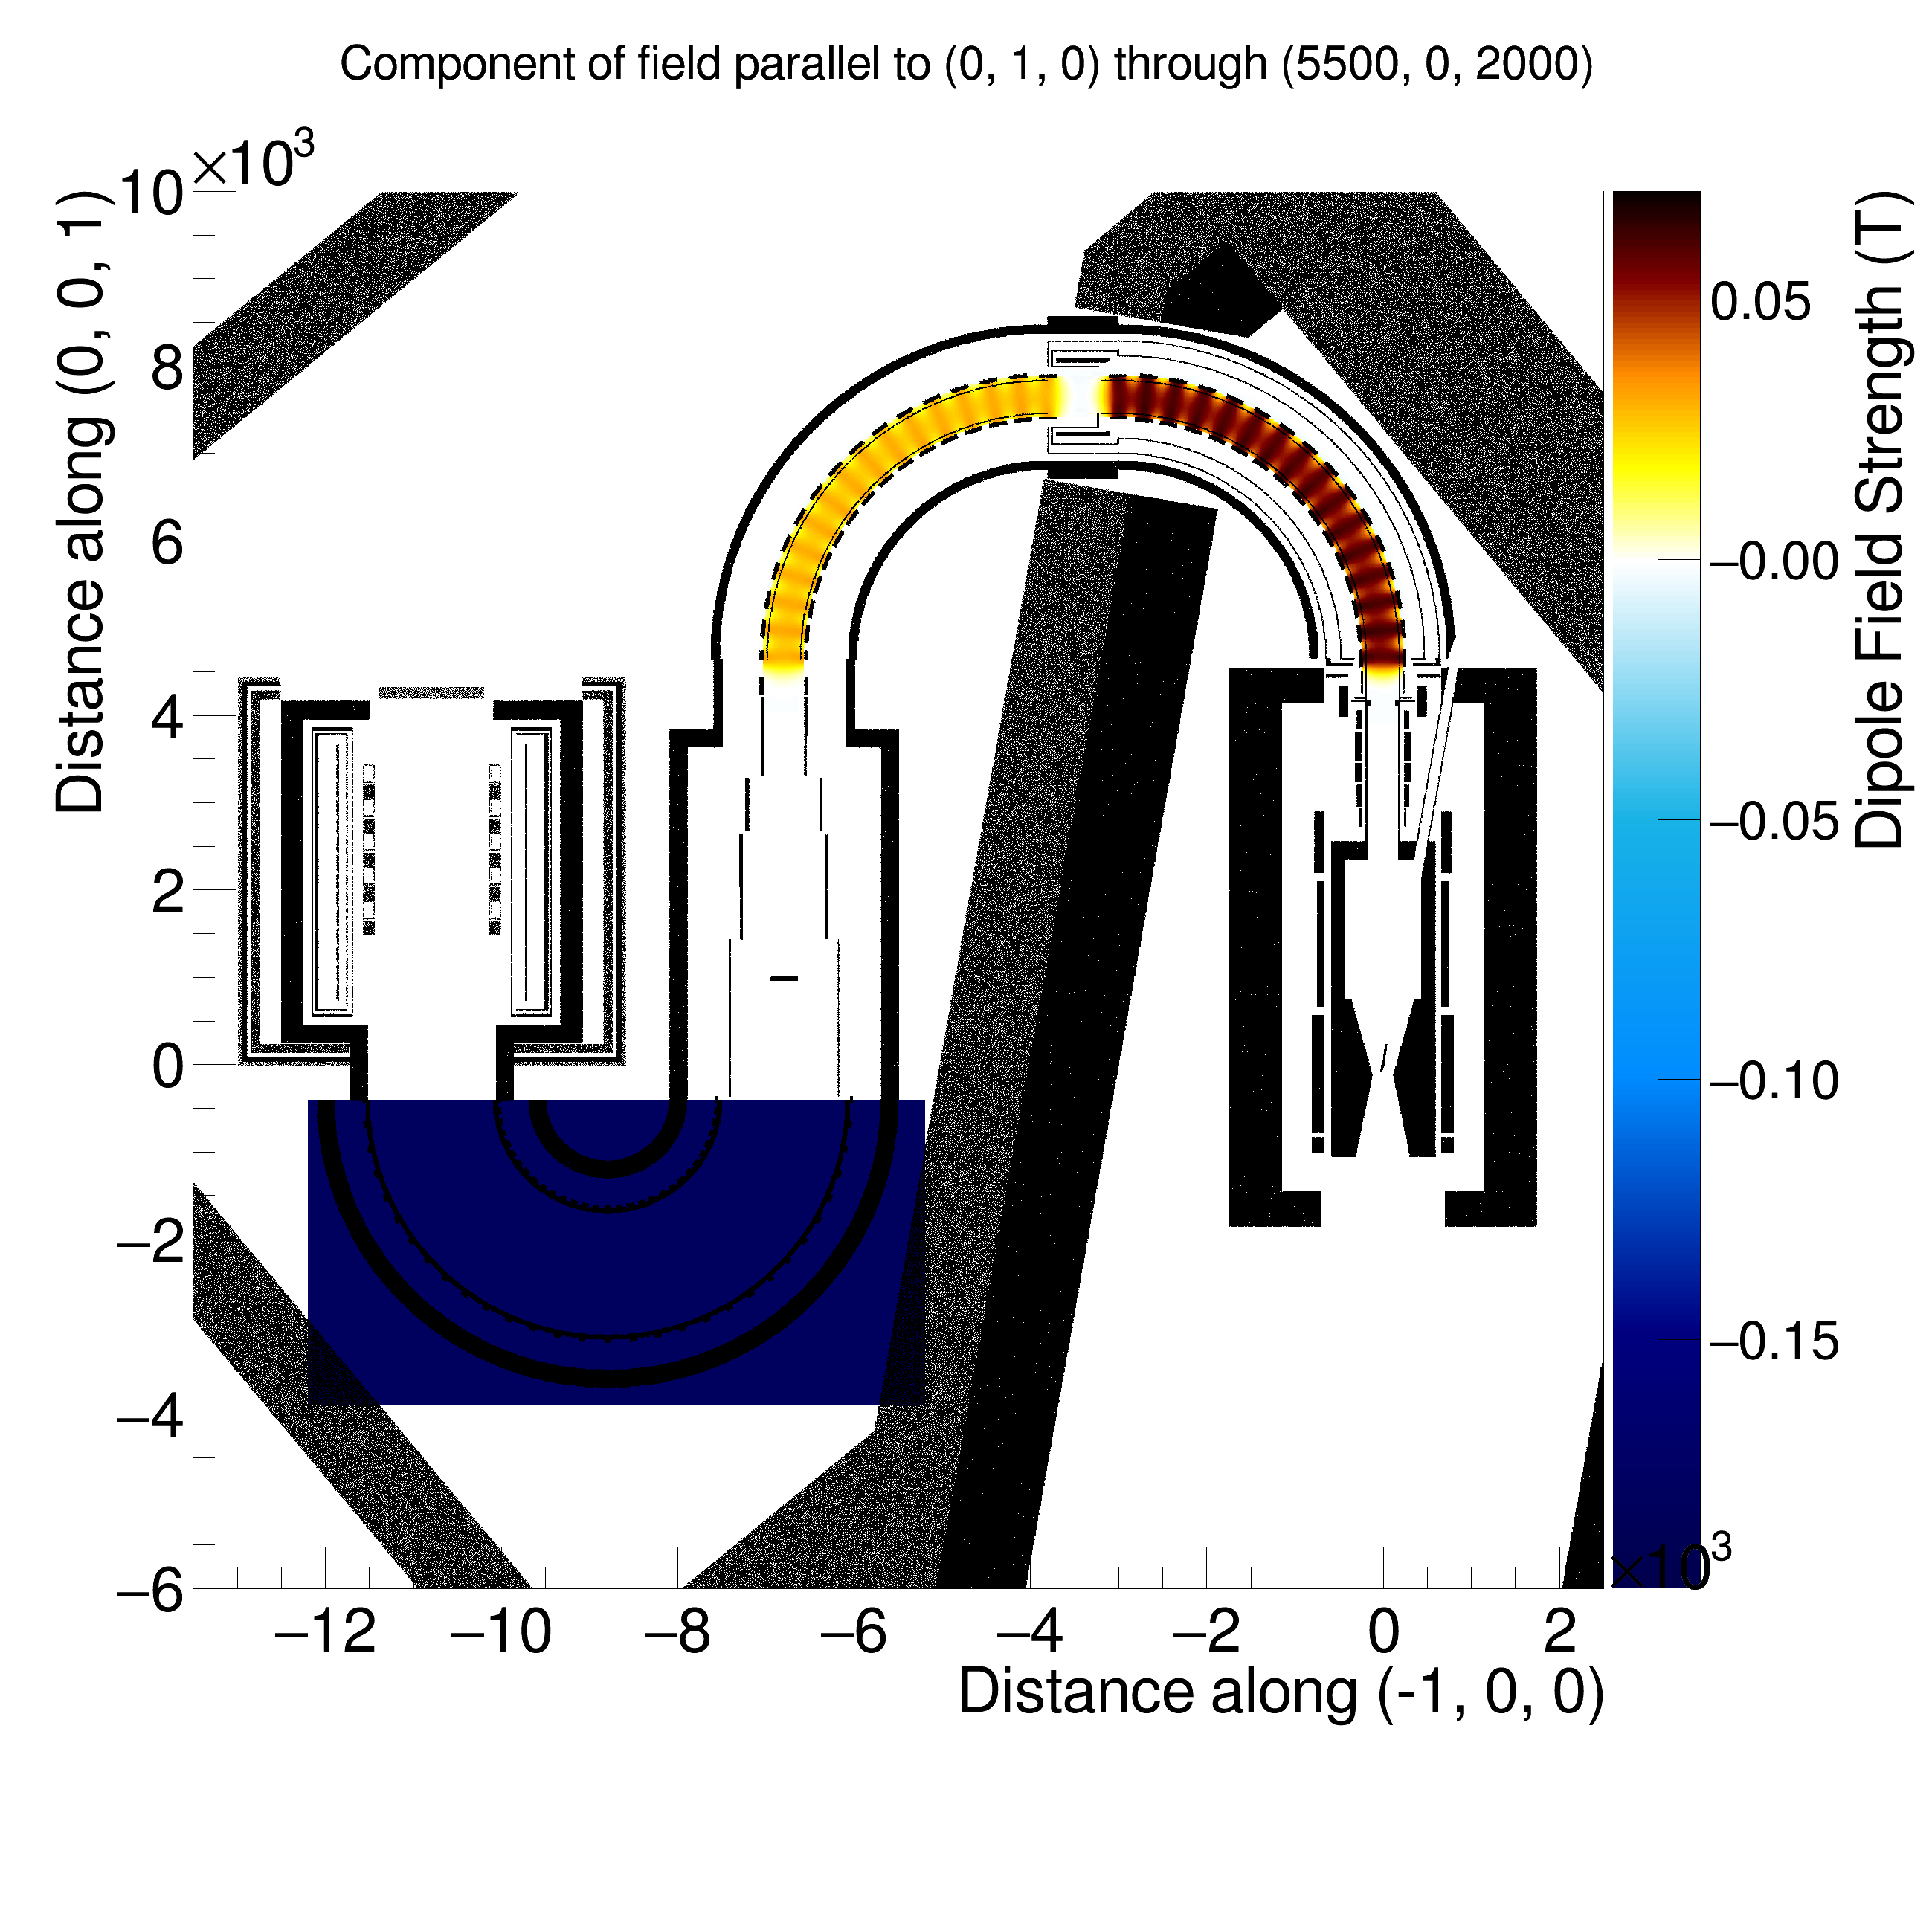
\includegraphics[width=0.9\textwidth,trim=2cm 8cm 0.0cm 6cm,clip=true]{figs/software/DipoleFields.png}
%}
\caption{
\figlabel{software:field:dipole}
The dipole field calculations used in ICEDUST for \phaseII. 
	The first 180\degree of the muon transport beamline have a positivie dipole field (pointing out of the plane)
	whilst the dipole along the electron spectrometer is negative and with a much larger strength.
	It can also be seen that the calculation for the dipole along the muon transport beamline contains realistic features (fringe fields, non-uniformities, etc)
	whilst the dipole field for the electron spectrometer is artificially uniform.  
}
\end{figure}
}

\chapter{Offline Software and The COMET Simulation}
In 2013, when I first worked on the COMET experiment, many disparate and stand-alone simulations were being used without a unified approach in the data structures and analysis.
Since then, a single unified software framework has been prepared and is now being used throughout the collaboration.
Developing this framework has been a large part of my work over the last four years, so this chapter presents both a summary of the framework and its development, as well as an explanation of the techniques used.

\section{Developing the COMET Offline Framework}
Work to produce a common, standardised software framework for COMET began when funding was awarded for \phaseI.
With some four years to go before the switch on, it was clear that the support structure to handle and analyse the data needed to be in place soon.
Given the scale of the project and the available resources, the decision was taken to base the COMET offline framework on an existing one, which would reduce the amount of work needed and improve the reliability of the software since it would have been tested elsewhere.
A requirements document was drawn up~\cite{ID:requirements} with a list of functionality that the software should provide.
A survey of existing experiments was then undertaken to build a list of candidate frameworks.
The list contained:
\begin{description}
\item [art] A framework being developed primarily at Fermilab~\cite{art:2011} which is also being used by Mu2e amongst other experiments.
\item [ND280] The framework~\cite{T2K:nim} used by the near detectors of the T2K experiment, which are also based at J-PARC.
\item [GAUDI] which is used by LHCb amongst other experiments~\cite{gaudi:2001}.
\item [MARLIN] The software being developed for the International Linear Collider (ILC)~\cite{marlin:web}.
\end{description}

The final decision was to use the ND280 framework\footnote{The term `ND280' can
refer to one of either the ND280 detector itself, the site at J-PARC that
houses both the ND280 and INGRID detectors, or the software used to analyse and
simulate the T2K near-detectors.  For the purposes of this chapter, unless
specified explicitly, the term `ND280' should be taken as referring to the
software.} 
since GAUDI and MARLIN would have required too much effort to adapt to the COMET
requirements; since art is a relatively new framework and will be used by Mu2e (keeping the software distinct is
important for the two experiments to co-exist as cross-checks); and because the
ND280 software was already known to a large part of the COMET collaboration and
had been tested, debugged, and used on real data at J-PARC.

\FigNDTwoEighty
\Fig{software:ND280} shows an overview of the ND280 framework, including its package structure and the various interactions between packages.

With the decision to base the COMET experiment on the ND280 framework---and with the selection of the new name: `ICEDUST'---the process of forking the software was begun.
As the ND280 framework had evolved somewhat organically, a review of the coding conventions was performed.
For example, whilst the ND280 software prefixes all classes with a capital `T', the ICEDUST conventions~\cite{ID:conventions} agreed to swap this to a capital `I' to reduce clashes with ROOT which also uses `T'.
The package renaming scheme~\cite{ID:ForkingDocs} was developed so that the purpose of a package and its role with the other packages could be more clearly identified.

Whilst fundamental, low-level packages have been left relatively unchanged, higher-level packages which include more detector-specific details had to be developed.
Additionally, some aspects of COMET needed considerably more support than had been present in the ND280 software.
Some of the key changes that have been introduced between ICEDUST and ND280 are:
\begin{description}
	\item [Simulation] Although the fundamental data types have not been changed, the simulation has been almost completely rewritten.
		In particular, support for hadron production codes have been added to model the production target;
		both the Geant4-based package (renamed to SimG4) and the detector response simulation (renamed as SimDetectorResponse) were given near-total makeovers;
		a new package (SimHitMerger) for resampling the G4Hits (simulated charge or energy deposits) was added.
		Custom physics models have been added to SimG4 to improve the modelling of the COMET-specific physics processes.
	\item [Magnetic Field handling]  Whilst the ND280 detector has a fairly straight-forward magnetic field, the COMET experiment has anything but this.  
		Accordingly, significant work has been made to replace the way
		the magnetic field was handled, from essentially a few constants
		to the ability to use complete fieldmap descriptions made with
		external field calculation software.
	\item [Geometry handling] The unusual shape of the COMET experiment, the level of detail needed for background estimations in a high-precision experiment, and the changing nature of a staged experiment meant a more elaborate scheme for handling the geometry was necessary than had existed in ND280.
	\item [Reconstruction and Calibration packages] The interdependence of the calibration and reconstruction packages has been refined, with the data flow and user interface being better defined and standardised.
		Additionally, support for track fitting using Genfit2~\cite{genfit-Hoppner:2009af} has been added as well as new track finding algorithms developed.
\end{description}

In addition to the above changes to the way the software runs, the distribution of the software has changed from using CMT~\cite{cmt} with CVS version control to being based on git with a GitLab~\cite{GitLab} web-based user interface for the official repository.
The switch to GitLab also brought a new `merge request' workflow, which has allowed development of ICEDUST to progress rapidly with only a small number of developers.
Although initially the intention was also to switch the build system from CMT to CMake~\cite{cmake}, this decision has since been reversed due to improvements in CMT.

In the 3 years since the summer of 2013 when the initial work to fork ND280 to ICEDUST, some 3,200 commits have edited about two million lines of code in the official version of the framework.
This has been the work of some 25 collaborators whilst about 15 other users have GitLab accounts and use the software.
ICEDUST has been used to run three large Monte Carlo productions, most recently simulating about $10^{11}$~\ac{POT} events---equivalent to 18,000 \phaseI bunches---and producing some 100~TB of simulated data.

\section{Overview of ICEDUST}
ICEDUST Can Efficiently Do Useful Software Things and stands for the Integrated COMET Experiment Data User Software Toolkit.
\Fig{software:ICEDUSTOverview} shows the flow of data through the different packages of the framework and the data formats used.

\FigICEDUSTOverview

Inside the framework, nearly all processing is done using a ROOT file-based format known as oaEvent.  
Files of this type contain header information providing run identification numbers as well as a description of the geometry and magnetic field.  
The data payload contained in oaEvent files is stored in a ROOT TTree with a single branch containing a single COMET event per entry.
Each COMET event has a dynamic structure and can contain any number of objects that derive from the IDatum base class.

Data from the detector systems is recorded in MIDAS~\cite{MIDAS} format, which also contains data from the slow control monitors such as temperature sensors and high-voltage power supplies.
The task of converting the MIDAS files into the oaEvent format is handled by the package oaUnpack, which writes out new, converted files, and oaRawEvent, which can convert the MIDAS files to oaEvent format on the fly.

Simulated data is also produced in the oaEvent format and involves some 4 to 6 packages being called, described in more depth in section~\sect{COMETSim}.

Once either simulated data has been produced or real data has been converted, calibration routines can then be applied.
Each sub-detector's routine is capable of pulling previously-generated constants from a MySQL database and applying these to the detected (or simulated) energy deposits.

These calibrated hits are then passed into the reconstruction stage.  
Here each sub-detector system is first allowed to handle the data, which is then passed to a global reconstruction routine until a fully reconstructed event is produced.
For the tracking detectors this stage typically involves an initial track finding stage, where noise hits are removed and track candidates consisting of a list of hits are collected and, secondly, a track fitting stage where the actual path of the underlying particle is reconstructed and key values like momentum and helical pitch-angle deduced.

Nearly all of the processing of data up to this stage has used the oaEvent format.
The final analysis stage, however, moves into a simpler, flatter format, known as oaAnalysis, which produces a data summary tree (as opposed to tape) that can be accessed without a dependence on the full ICEDUST software.

Around all of this there are several utility packages such as the event display, which can visualise any oaEvent file, and IcedustControl, which can run a single set of data through the data chain and is the main steering mechanism used for production running.

\section{The COMET Simulation}
\sectlabel{COMETSim}
During \phaseI and \phaseI some $10^{19}$ and $10^{21}$ protons will strike the production target.
Of these, fewer than 1 background events should be observed, whilst the signal efficiency should be demonstrably as high as possible.
%
%The ability for an experiment to set stringent confidence limits in the event of a null-observation is determined both by the expected signal acceptance (which should be high) and the predicted number of background events (which should be low).
%For COMET's target single-event sensitivity---which is only a measure of the signal efficiency---to translate to a comparable confidence limit if no signal is observed, less than one background events should be expected during the entire run.
%By comparison, some $10^{19}$ and $10^{21}$~protons will impinge the production target in \phaseI and \phaseII respectively, so it is clear that the ability to suppress backgrounds must be demonstrably high.

Simulation plays a crucial role in making such a demonstration. 
Before the experiment is built and operated it allows one to optimise crucial aspects of the geometry and parameters, such as the magnetic field strengths or timing cuts.
In addition, using Monte Carlo techniques in an accurate simulation allows an estimation of the background rate by sampling the parameter space corresponding to each stage of the experiment.
Clearly, then, the simulation itself must be as faithful a reproduction of the true experiment as possible.
\FigSimulationOverview

The COMET simulation therefore needs to be both highly accurate and highly efficient.
As well as custom physics modelling, and special handling for the magnetic field, several resampling techniques have been introduced to increase the statistical power.
The steps needed to build up the COMET simulation are shown in \fig{software:SimulationOverview}.

To reduce the uncertainties associated with the production target and the muon and pion yield multiple hadron codes can be used, including PHITS~\cite{PHITS2002}, MARS~\cite{MARS1995}, Fluka~\cite{FLUKA2005} and Geant4~\cite{Geant42003}.
The SimG4 package, which is based on Geant4, then takes over the muon beam simulation and tracking of particles to the detectors.
These energy deposits, referred to as G4Hits, can then be converted to realistic electronic detector-readouts by the SimDetectorResponse package.
On most occasions, though, the G4Hits are first reshuffled with G4Hits from other \acf{POT} events so that a realistic bunch structure is built up and processed, since it is this structure that the true detector will see.
SimG4 produces one output event for every primary vertex introduced\footnote{This typically means one output event per proton-on-target, but in principle could be something else, such as one output event per signal electron in a dedicated trigger simulation}, %
whereas SimDetectorResponse needs to produce the same sort of data structure as will be seen in the real experiment, which is one event per proton bunch.

This requires some intermediate step, known as the SimHitMerger, to shuffle the events from SimG4 together and build up realistic bunch events.
This is one point where a degree of resampling is introduced, since there are virtually no correlations between proton events.
Within a SimG4 output event all timing is given with respect to the original primary vertex.  
Since protons on target are introduced at $t=0$, all G4Hits have their timing given with respect to the proton arriving at the production target.
In the process of building bunch events, a realistic timing structure for the proton beam is introduced by shifting the time of all hits for a given proton event by a fixed amount, as if the proton had arrived slightly earlier or later.

A bunch event in \phaseI will consist of about \num{8e6}~\acp{POT} so, without resampling, a simulation of 8$\times10^{8}$~\ac{POT} events, for example, could only produce 100 bunches.
Since the proton events are uncorrelated, by picking different proton events and applying different time shifts to each one it is possible, in principle, to build a much larger number of bunch events.

An additional form of resampling can also be used during the Geant4 simulation, by dividing up the experiment into different stages and restarting the simulation multiple times at a later stage, reusing the output from the earlier section.
For example, a simulation of the production target region is used to track particles up to the boundary of the muon beam line.
The muon beam simulation is then repeated multiple times using the particles that left the production target section as an input and changing the initial random seed for each restart.
This technique was used in the most recent large scale mass production twice---once at the production target section and again at the entrance to the detector solenoid region---restarting the simulation five times for each section, so that for each initial proton on target, 25 times this number of events were tracked through the detector solenoid.

Both of these resampling techniques must be handled with care since this can produce correlations between the events produced from resampled inputs.
Reconstruction methods often employ machine learning techniques which are particularly sensitive to correlations within a dataset.
To reduce any potential impact due to resampling, the resampled data is handled in distinct sets so that within a set no proton on target event is repeated in more than one output bunch event.

\subsection{Handling Geometry}
During the change from ND280 to ICEDUST, a new geometry handling scheme was introduced to the SimG4 package.
This change was motivated by: 
    the fact that COMET has a large number of components with a large variety of complexities, shapes, and sizes;
    the COMET geometry will change dramatically throughout the lifetime of the experiment;
    all pieces of material close to the beam could potentially contribute to background rates if, for example, they scatter high energy particles into a high-acceptance region of phase space.

The aim of the new geometry handling scheme tries to address these issues.
The goals in developing the new approach were to:
\begin{itemize}
\setlength{\itemsep}{-1ex}
\item define a clear mechanism for how the geometry is implemented and controlled;
\item decouple the code for physically isolated parts of the experiment;
\item provide the flexibility to add and remove parts of the experiment;
\item maximise the maintainability of the code related to geometry;
\item allow for easy inspection of both the geometry and the various parameters that control it.
\end{itemize}

\FigGeometryHeirarchy

The final scheme uses a nested component structure, which is built up using compiled c++ to define the volume hierarchy in a modular way, with parameters provided at run-time to define the actual shapes and locations of the volumes.
The run-time parameters are `owned' by the component they are attributed to and can be assigned values based on that of other parameters and inspected easily by various print commands.
Access to the values of other parameters is possible if and only if they are owned by an accessible component.
Whether or not another component is accessible depends on its relative position in the component hierarchy: the target component must either be an ancestor, immediate child, or share the same parent component, as demonstrated in \fig{software:componentHeirarchy}.

To provide the value of a parameter, standard, human-readable, infix notation allows arithmetic between integers, floating point numbers, three-vectors, and rotation matrices.
In addition, parameters can be easily repeated or indexed, such as for the positions of crystals in the ECAL or straws in a straw tracker plane, where the $i$\textsuperscript{th} position depends on the value of $i$.
A demonstration of valid parameter assignments is shown in \fig{software:geom:paramAssignments}.

\FigGeometryParameters
\FigGeometryScreenshots

Using this scheme, multiple `worlds' have been developed corresponding to different stages and run-configurations of COMET, between which a user can easily change.
Each world is able to re-use much of the code for another, such as the experiment hall building, which appears in every world.
In addition, it has been straight forward to build up significant complexity in key areas such as the production target.
\Fig{software:geom:screenshots} shows two of the available worlds that have been created using this scheme.

A more thorough description of the geometry scheme  in SimG4, as well as a users guide and walk-through, can be found at \url{www.hep.ph.ic.ac.uk/~bek07/comet/SimG4/documentation/index.shtml}.

Once SimG4 has created the geometry, it writes it out to a ROOT-based format alongside the data, using ROOT's TGeo classes~\cite{ROOTTGeo}.
This is then used by the other packages, such as calibration and analysis.  
The event display also uses this to show the various hits and tracks overlaid on the geometry.

\subsection{Field Calculation}
\sectlabel{sw:fieldmap}
%\begin{easylist}
%%# In COMET a static magnetic field is used to capture and disperse charged particles.
%%# Bumps in field can mirror particles which will cause delays to particle arrival
%%# Need dipole field and solenoid field calculations
%# Calculations by Toshiba, and in-house using Opera, Tosca and G4Beamline.
%# Handling of fieldmap information in ICEDUST
%# Although pure magnetic fields are currently used, electric fields can in principle be added in exactly the same way.
%\end{easylist}

An essential aspect of the \COMET experiment is the static magnetic field that is used along the beam line to capture, focus, or disperse charged particles.
Modelling this field accurately is important to ensure any outcomes of the simulation are reliable.
In particular, local reductions in the field strength risk mirroring particles backwards or even trapping particles for extended periods.
This could be especially dangerous for \COMET since, in the process, the timing information of the particle is lost, reducing the effectiveness of the timing cut to suppress backgrounds.

Magnetic field calculations can become quite computationally expensive.  
As a result, approximations and assumptions are often made to simplify the process, such as the assumption of symmetry about an axis or plane to reduce the effective number of dimensions to the problem.
As well as modelling the current in the coils, material effects should also be accounted for, particularly in the yoke and surrounding material of the beamline.
Often these material effects are linear, but in regions of high magnetic field this linearity can be lost via processes such as saturation, further increasing the computational complexity.

There are two distinct types of magnetic field used in COMET: a solenoidal field produced by a winding of superconducting cable in a spiral, and that of the dipole fields, which are produced by a novel winding technique that
is proprietary to Toshiba.  
Although there are several areas of `bent' solenoid, these are actually formed by a series of smaller straight solenoid sections and so do not need special treatment in the field calculation.
Straight solenoids are used in many other applications such that existing coil calculation methods are reliable. 
Calculating the dipole field, however, is not so straightforward since the exact configuration is owned by Toshiba.

The COMET collaboration have used several different methods to perform field map calculations.
G4Beamline~\cite{G4Beamline} is a simulation toolkit that makes numerous extensions to Geant4 and is able to perform simple solenoid calculations directly.
Whilst it cannot model material effects, its speed and simplicity allows quick and simple studies. 
The methods for solenoid calculations of this open-source project have been incorporated into SimG4, so that the package can directly produce the field for solenoid coils contained in its geometry.
The resultant fieldmap is shown in \fig{software:field:G4Beamline}.
\FigSoftwareFieldMap
\FigSoftwareFieldMapComparison

For more elaborate calculations, Opera 3D finite-element-analysis software was used with the TOSCA sub-module~\cite{Opera} for static electromagnetic fields.
This calculation includes non-linear material effects in the yoke and shielding so that the final fieldmap should be much more accurate.
\Fig{software:field:Opera} shows the fieldmap calculated by Opera in the plane of the beam line axis.
The ratio between the G4Beamline and Opera calculations is given in \fig{software:field:comparison}, where it can be seen how the two models disagree most at the exit of the solenoids.

Whilst the above two methods have been used for the solenoid fields, calculating the dipole field structure is a different story, given that the winding is proprietary information belonging to Toshiba.
For the dipoles in the muon beamline Toshiba have provided a calculation for one octant of one winding, which is then mirrored and placed multiple times along the beamline.
For the dipoles along the electron spectrometer of \phaseII there is no accurate calculation at this time.

Whilst only magnetic fields have been used in the simulation up to now, ICEDUST is able to handle electric fields in exactly the same way.
For instance future work might see the electric fields for the straw tracker and CDC included to account for the impact that these fields might have on particle scattering in the detector.

Field map files are treated as a single data file which are loaded in and placed with a given rotation and translation as well as an overall field scale factor.
It is important that subsequent processing of data files be able to reproduce the same field as used to generate the data.
Since many individual field map files are often loaded in to assemble an overall representation of the field to facilitate such book-keeping, a description of each of the used fieldmap files is stored alongside the data, in a similar way to the geometry.
This information contains the name and a check-sum for the original fieldmap file as well as the rotation, translation, and scale factor.
Given a data file and the location of a directory containing the fieldmap files, all ICEDUST programs are, therefore, able to re-instantiate the field.
Other types of field component, such as the solenoid fields produced with the incorporated G4Beamline code, are also persisted and re-instantiated in this manner.

\subsection{Production Target Simulations}
\FigPiYieldHadronCodes
There is currently a lack of experimental data for interactions of protons with 8~GeV kinetic energy with a tungsten target, especially for production of negative pions in the backwards direction.
\Fig{detector:piYield} seems to be the best source of experimental data, but even this is problematic in that it represents 10.1~GeV protons striking a tantalum target and that the actual data points are not tabulated anywhere in the literature.

The HARP experiment~\cite{HARP2007} has also measured pion yields in the context of future neutrino beam facilities and have used an 8~GeV proton beam with a tungsten target
Unfortunately they only observed pion yields at angles of less than around 2 radians for such a combination of target and proton energy.

As a result of this shortage of measured values, it is important to use as many hadron models as possible to pin down the uncertainty on the predicted pion and muon yield.
Previous studies have compared the HARP data to predictions from several hadron codes~\cite{AEdmondsThesis,YeYangPrivate} some of which are reproduced in \fig{software:piYield}.
From these it is clear that no one model can reproduce the experimental data accurately for all angular regions and all materials.

Currently, PHITS~\cite{PHITS2002}, MARS~\cite{MARS1995}, Fluka~\cite{FLUKA2005}, and Geant4~\cite{Geant42003} can all be used to run production target simulations and feed results into the rest of the experiment.
The level of integration of these packages varies, however.
SimG4 (which is based on Geant4) and SimMARS (which interfaces MARS into ICEDUST) are able to read directly the standard ICEDUST geometry and fieldmap formats and they are able to output directly to a format known as oaRooTracker, which the SimG4 package is able to read back in.
On the other hand, both Fluka and PHITS (interfaced via SimFluka and SimPHITS, respectively)  are written in Fortran and have proved harder to integrate. 
At this point in time, each must separately produce the geometry and fieldmap and have their outputs post-converted to the oaRooTracker format.  
Fluka also lacks a primitive Torus volume implementation, so that other studies such as neutron rates are further limited in Fluka at this stage.

\subsection{Extending the Geant4 Physics Modelling}
%\begin{easylist}
%# Geant4 is the main library used to track particles from the production target to the detectors.
%# Uses modular physics lists to run the possible interactions of a particle, either along a step in the tracking, at the end of a step or once the particle has come to rest in some material.
%# SimG4 builds on the physics list known as \_\_\_\_
%# This list defines models for ....
%%# Aside from the production target, which has already been discussed, crucial physics process for COMET are: Muon nuclear capture, muon decay in orbit, pion radiative capture
%# Modelling processes stopped negative muons is crucial to simulating COMET.
%	# The standard handling of a stopped negative muon is to decide whether the muon is captured or decayed, then apply specific implementations for these processes .... (pseudo-code for G4 algorithm?)
%	# DIO is treated as a crude variation of the free muon decay, such that an end-point in the spectrum occurs well below the true end-point
%	# Comparison of default Geant4 vs. Czarnecki et al paper
%	# RMC is treated as a Bertini cascade where the incoming projectile has the mass of a muon.  
%	# Bertini cascade was developed on data for pion capture, and is likely a bad model for the capture of a muon, since a muon undergoes no strong interactions within the nucleus.
%	# Alcap experiment has measured products from RMC and additional data can be found.
%	# Comparison of default Geant4 vs. RMC spectrum from Alcap
%	# In addition to modifying the physics processes for capture and decay, also need to include conversion in the simulation.
%	# Extension to Geant4 classes to inject custom DIO and muon capture spectra.
%	# New pseudo code for running negative stopped muon processes
%	# Additional models that should be added in the future:
%	## Antiprotons, RPC, DIO and capture on other materials
%\end{easylist}

\subsubsection{Geant4 physics modelling}
Aside from the production target region, most of the tracking of particles and creation of secondaries takes place in the SimG4 package, which is built against the Geant4 library.
In Geant4, the trajectory of a particle is built up in steps, each of which terminates either by a physics process (which might change the particle's direction or energy, or produce secondary tracks) or by the boundary of a volume in the simulated geometry.
To decide what actually limits the step taken by a given particle (a positron, for example ), Geant4 calls the list of possible processes this particle can undergo (for example Bremsstrahlung, annihilation, inverse Compton scattering, etc) and asks each process for a proposed step length. 
In the case of a geometry limit, the step length is the distance until the boundary of the geometry, including deflections to the trajectory due to any electromagnetic field.
On the other hand, for a physics process the proposed step length is typically selected randomly using a relevant probability distribution for this process.
Often this involves a characteristic length or time of the process, for example the half-life of a particle that will decay.
Out of all possible step limits, the process proposing the shortest limit (or, if the particle is at rest, the soonest limit) is chosen.
The current position and momentum of the particle is updated accordingly and any secondary particles produced are prepared for tracking.

\FigSoftwarePhysicsSpectra
Determining which processes are applied to which particles and how each process is modelled is an important part of building a Geant4 simulation; the library provides a list of standard physics lists to help the process.
Choosing the right physics list depends on the goal of the simulation, for example which particles are involved; what energy ranges are interesting; and which background effects must be included.
To simulate \COMET the QGSP\_BERT\_HP physics list~\cite{Geant4:QGSP-BERT} was chosen as a starting point.
This model is expected to perform well for low energy dosimetry, shielding, and neutron calculations~\cite{Geant4:PhysicsListsRecommends}.

On top of this physics list, custom changes have been made to the way negative muons are treated once stopped in material.
COMET is somewhat unusual in the field of modern particle physics for dealing with muons at very low energy, unlike at the \ac{CERN} experiments, for example, where they are normally treated as minimally-ionising particles (MIPs).
As a result,  the modelling of low-energy negative muons is relatively simplistic in the default physics processes of Geant4.
In addition to this, for the COMET experiment it is important to add the process of coherent \mueconv, which, as a currently unobserved process, is not included in Geant4.

In the \ac{SM}, a stopped negative muon that has been captured to an atomic orbital can either undergo decay or nuclear capture.
As previously discussed, the end-point for electrons coming from muon \ac{DIO} reaches up to the \mueconv limit, or around 105~MeV/c.  
Vanilla Geant4, however, is unable to produce this tail, and on aluminium is only able to produce electrons up to around 60 MeV/c.  
This is because the bound muon decay model in Geant4 uses the free muon decay spectrum and applies a boost in a random direction, with the boost factor set by the muon binding energy.
A comparison of the electron spectrum from this model and that proposed by Czarnecki \etal~\cite{Czarnecki2011} is shown in \fig{software:customPhysic:DIO}, where it can be seen how the high energy tail falls far more rapidly in the Geant4 spectrum.

Similarly, for the nuclear capture of the muon, there are sizeable disagreements between the available (but limited) data and the default Geant4 model.
For example, the AlCap experiment~\cite{AlcapProposal2012} has improved the knowledge of proton emission following muon nuclear capture in aluminium.
This showed that proton emission occurs for around 3~\% of all nuclear captured muons; Geant4 produces around around 7 to 8 times more than this.
The overall shapes of the proton spectra also disagree.
Although the AlCap result is still only preliminary, the spectrum that has been observed is much softer than that produced by standard Geant4, as shown in \fig{software:customPhysic:ProtMuCap}.

Standard Geant4 models nuclear capture of negative muons using a Bertini cascade which was developed using incident hadrons~\cite{Geant4:Bertini}.
Muon nuclear capture is thought to occur via a combination of direct capture on a proton, producing a neutron, or via an interaction with a set of clustered nucleons.
The latter is typically invoked to explain proton emission.
The Bertini cascade model handles negative muon capture by first handling the prompt process of muon capture on the nucleons, then cascading the resultant nucleons through the nucleus.
A point within the nucleus is chosen homogeneously and then the muon interacted with either a single proton or a nucleon pair.
It is not clear, at this stage, what causes the discrepancy between this model and the experimentally observed result for proton emissions.

\subsubsection{Extending the physics processes}
To resolve these issues, custom physics classes have been added to the \COMET simulation.
The key design goal of these classes was to allow future improvements in the experimental and theoretical inputs to be added, yet decouple the implementation from the normal Geant4 implementation so that future updates to Geant4 could easily be absorbed.

\Fig{software:ExtendedMuonClasses} shows the class interaction diagram for the extended physics modelling for stopped negative muons.
The standard Geant4 model sets up these processes using the `G4MuonMinusCapture' class, which passes concrete implementations for decay and nuclear capture into its base-class `G4HadronStoppingProcess'.
This base-class contains three instances of a `G4HadronicInteraction': one to perform the electromagnetic cascade between the atomic orbitals; another to perform \ac{DIO}; and a third to perform the nuclear capture.
The `G4HadronStoppingProcess' class is also used to simulate stopped negative pions, kaons, and so on, and bound decay is only considered if a valid instance of such a process has been provided.
When a stopped particle is processed through this class, the electromagnetic cascade is always run first, producing X-rays and Auger electrons.
Then one of either bound decay or nuclear capture is chosen by asking the bound decay process whether or not it will kill the particle; if so, bound decay is considered to have taken place and the nuclear capture is not run. 
Default Geant4 uses nuclear capture rates based on a 1987 paper by Suzuki \etal~\cite{Suzuki1987}  which fill in experimental blanks with a semi-empirical models, and decay rates based on a largely theoretical 1977 model by Mukhopadhyay~\cite{Mukhopadhyay:1976hu}.
\Fig{detector:mu-nucl-params} was produced by extracting these parameters.

\FigSimulationPhysicsClasses
To extend the default Geant4 modelling and improve the accuracy with the improved theoretical understanding of the \ac{DIO} process and measurements of muon nuclear capture, three new classes have been written which mirror the way the default Geant4 model is implemented but add more detail.
These new classes are shown in \fig{software:ExtendedMuonClasses} in red.  
Currently they only play a role if the muon stops in aluminium otherwise they invoke directly the default Geant4 model.
`COMETMuonMinusBoundDecayOrConversion' takes over the task of bound decay by first deciding whether to capture, decay, or convert based on rates which can be adjusted at run-time by Geant4 commands.
The default rates are the normal Geant4 rates of capture and decay and a conversion rate of $10^{-15}$ (which is multiplied by the capture rate to get the total conversion branching ratio).
If the conversion process is chosen, an electron with total energy of 104.97~MeV is produced in a random direction.  
If decay is chosen, a \ac{DIO} spectrum is used to randomly generate an energy, which at the time of writing defaults to the 2011 Czarnecki spectrum~\cite{Czarnecki2011}, although other spectra can be specified at run-time.
If neither of these processes are selected, then the `COMETMuonMinusBoundDecayOrConversion' class returns, leaving the muon status as alive such that the capture process takes place.
At this point, control would pass to the `COMETMuonMinusCapture' class, which contains an instance of the default Geant4 Bertini Cascade model to use for materials other than aluminium.
Run-time controls allow the default model to be re-enabled for aluminium.

The `COMETMuonMinusCapture' class contains a list of types of secondary particle which it is able to produce.  
For each possible secondary, both a total production rate per capture and spectrum must be supplied.
When a muon captures in aluminium, firstly the default model is run.
Then, for each of the secondaries produced by this, if a custom rate and spectrum have been provided for a particle of this type, the secondary from the Bertini cascade is removed.
Next, for each of the particles that do have custom rates and spectra, a particle is produced with the given probability and each of these particles assigned an energy given randomly according to the selected spectrum.
By using the default model first, particles for which experimental rates or spectra do not exist can still be produced in the simulation.

There are, however, some downsides to this approach.
Although the remnant nucleus is not actually tracked, in principle energy conservation is not guaranteed since the custom models do not work with the default model to ensure this.
In addition, the custom models cannot simulate correlations between different particle types. 
For example, the probability of emitting a neutron or gamma particle might be dependent on whether or not an alpha particle is emitted. 
Although such details cannot be included in this modelling, the impact to the outputs of the simulation are expected to be small, if not negligible, since the detector will see particles from hundreds of thousands of stopped muons per bunch, and will not look at the correlations between different particle types.

Finally, to handle the various spectra that might be added to the simulation, a special spectrum and spectrum-factory class design was added.
The `COMETVSpectrum' base-class was added to represent the abstract idea of a 1-dimensional spectrum.
Custom spectra, such as the Czarnecki \ac{DIO} spectrum or the AlCap protons from muon capture spectrum, can be included by writing a concrete instance of a spectrum, derived from `COMETVSpectrum'.
Custom physics processes can use these spectra as they like, and since the `COMETSpectrumFactory' class is able to produce concrete spectra when given a string with the name of the desired spectrum, the custom physics models can easily have different spectra selected by run-time commands.
In addition, a new primary particle generator has been added which allows the momentum or energy of a particle to be set according to a named spectrum, which will be identical to the spectrum used in the tracking process.
This makes it easy  to run specific acceptance studies and also reduces the effort needed to add a new physics model since one spectrum can be written and immediately used by both the primary event generators and the tracking physics.

%\subsection{Resampling With the Hit Merger}
